% uWaterloo Thesis Template for LaTeX 
% Last Updated June 14, 2017 by Stephen Carr, IST Client Services
% FOR ASSISTANCE, please send mail to rt-IST-CSmathsci@ist.uwaterloo.ca

% Effective October 2006, the University of Waterloo 
% requires electronic thesis submission. See the uWaterloo thesis regulations at
% https://uwaterloo.ca/graduate-studies/thesis.

% DON'T FORGET TO ADD YOUR OWN NAME AND TITLE in the "hyperref" package
% configuration below. THIS INFORMATION GETS EMBEDDED IN THE PDF FINAL PDF DOCUMENT.
% You can view the information if you view Properties of the PDF document.

% Many faculties/departments also require one or more printed
% copies. This template attempts to satisfy both types of output. 
% It is based on the standard "book" document class which provides all necessary 
% sectioning structures and allows multi-part theses.

% DISCLAIMER
% To the best of our knowledge, this template satisfies the current uWaterloo requirements.
% However, it is your responsibility to assure that you have met all 
% requirements of the University and your particular department.
% Many thanks for the feedback from many graduates that assisted the development of this template.

% -----------------------------------------------------------------------

% By default, output is produced that is geared toward generating a PDF 
% version optimized for viewing on an electronic display, including 
% hyperlinks within the PDF.
 
% E.g. to process a thesis called "mythesis.tex" based on this template, run:

% pdflatex mythesis	-- first pass of the pdflatex processor
% bibtex mythesis	-- generates bibliography from .bib data file(s)
% makeindex         -- should be run only if an index is used 
% pdflatex mythesis	-- fixes numbering in cross-references, bibliographic references, glossaries, index, etc.
% pdflatex mythesis	-- fixes numbering in cross-references, bibliographic references, glossaries, index, etc.

% If you use the recommended LaTeX editor, Texmaker, you would open the mythesis.tex
% file, then click the PDFLaTeX button. Then run BibTeX (under the Tools menu).
% Then click the PDFLaTeX button two more times. If you have an index as well,
% you'll need to run MakeIndex from the Tools menu as well, before running pdflatex
% the last two times.

% N.B. The "pdftex" program allows graphics in the following formats to be
% included with the "\includegraphics" command: PNG, PDF, JPEG, TIFF
% Tip 1: Generate your figures and photos in the size you want them to appear
% in your thesis, rather than scaling them with \includegraphics options.
% Tip 2: Any drawings you do should be in scalable vector graphic formats: SVG, PNG, WMF, EPS and then converted to PNG or PDF, so they are scalable in
% the final PDF as well.
% Tip 3: Photographs should be cropped and compressed so as not to be too large.

% To create a PDF output that is optimized for double-sided printing: 
%
% 1) comment-out the \documentclass statement in the preamble below, and
% un-comment the second \documentclass line.
%
% 2) change the value assigned below to the boolean variable
% "PrintVersion" from "false" to "true".

% --------------------- Start of Document Preamble -----------------------

% Specify the document class, default style attributes, and page dimensions
% For hyperlinked PDF, suitable for viewing on a computer, use this:
\documentclass[letterpaper,12pt,titlepage,oneside,final]{book}
 
% For PDF, suitable for double-sided printing, change the PrintVersion variable below
% to "true" and use this \documentclass line instead of the one above:
%\documentclass[letterpaper,12pt,titlepage,openright,twoside,final]{book}

% Some LaTeX commands I define for my own nomenclature.
% If you have to, it's better to change nomenclature once here than in a 
% million places throughout your thesis!
\newcommand{\package}[1]{\textbf{#1}} % package names in bold text
\newcommand{\cmmd}[1]{\textbackslash\texttt{#1}} % command name in tt font 
\newcommand{\href}[1]{#1} % does nothing, but defines the command so the
    % print-optimized version will ignore \href tags (redefined by hyperref pkg).
%\newcommand{\texorpdfstring}[2]{#1} % does nothing, but defines the command
% Anything defined here may be redefined by packages added below...

% This package allows if-then-else control structures.
\usepackage{ifthen}
\newboolean{PrintVersion}
\setboolean{PrintVersion}{false} 
% CHANGE THIS VALUE TO "true" as necessary, to improve printed results for hard copies
% by overriding some options of the hyperref package below.

%\usepackage{nomencl} % For a nomenclature (optional; available from ctan.org)
\usepackage{amsmath,amssymb,amstext} % Lots of math symbols and environments
\usepackage[pdftex]{graphicx} % For including graphics N.B. pdftex graphics driver 

% Hyperlinks make it very easy to navigate an electronic document.
% In addition, this is where you should specify the thesis title
% and author as they appear in the properties of the PDF document.
% Use the "hyperref" package 
% N.B. HYPERREF MUST BE THE LAST PACKAGE LOADED; ADD ADDITIONAL PKGS ABOVE
\usepackage[pdftex,pagebackref=false]{hyperref} % with basic options
		% N.B. pagebackref=true provides links back from the References to the body text. This can cause trouble for printing.
\hypersetup{
    plainpages=false,       % needed if Roman numbers in frontpages
    unicode=false,          % non-Latin characters in Acrobat’s bookmarks
    pdftoolbar=true,        % show Acrobat’s toolbar?
    pdfmenubar=true,        % show Acrobat’s menu?
    pdffitwindow=false,     % window fit to page when opened
    pdfstartview={FitH},    % fits the width of the page to the window
    pdftitle={uWaterloo\ LaTeX\ Thesis\ Template},    % title: CHANGE THIS TEXT!
%    pdfauthor={Author},    % author: CHANGE THIS TEXT! and uncomment this line
%    pdfsubject={Subject},  % subject: CHANGE THIS TEXT! and uncomment this line
%    pdfkeywords={keyword1} {key2} {key3}, % list of keywords, and uncomment this line if desired
    pdfnewwindow=true,      % links in new window
    colorlinks=true,        % false: boxed links; true: colored links
    linkcolor=blue,         % color of internal links
    citecolor=green,        % color of links to bibliography
    filecolor=magenta,      % color of file links
    urlcolor=cyan           % color of external links
}
\ifthenelse{\boolean{PrintVersion}}{   % for improved print quality, change some hyperref options
\hypersetup{	% override some previously defined hyperref options
%    colorlinks,%
    citecolor=black,%
    filecolor=black,%
    linkcolor=black,%
    urlcolor=black}
}{} % end of ifthenelse (no else)

\usepackage[automake,toc,abbreviations]{glossaries-extra} % Exception to the rule of hyperref being the last add-on package
% If glossaries-extra is not in your LaTeX distribution, get it from CTAN (http://ctan.org/pkg/glossaries-extra), 
% although it's supposed to be in both the TeX Live and MikTeX distributions. There are also documentation and 
% installation instructions there.

% Setting up the page margins...
% uWaterloo thesis requirements specify a minimum of 1 inch (72pt) margin at the
% top, bottom, and outside page edges and a 1.125 in. (81pt) gutter
% margin (on binding side). While this is not an issue for electronic
% viewing, a PDF may be printed, and so we have the same page layout for
% both printed and electronic versions, we leave the gutter margin in.
% Set margins to minimum permitted by uWaterloo thesis regulations:
\setlength{\marginparwidth}{0pt} % width of margin notes
% N.B. If margin notes are used, you must adjust \textwidth, \marginparwidth
% and \marginparsep so that the space left between the margin notes and page
% edge is less than 15 mm (0.6 in.)
\setlength{\marginparsep}{0pt} % width of space between body text and margin notes
\setlength{\evensidemargin}{0.125in} % Adds 1/8 in. to binding side of all 
% even-numbered pages when the "twoside" printing option is selected
\setlength{\oddsidemargin}{0.125in} % Adds 1/8 in. to the left of all pages
% when "oneside" printing is selected, and to the left of all odd-numbered
% pages when "twoside" printing is selected
\setlength{\textwidth}{6.375in} % assuming US letter paper (8.5 in. x 11 in.) and 
% side margins as above
\raggedbottom

% The following statement specifies the amount of space between
% paragraphs. Other reasonable specifications are \bigskipamount and \smallskipamount.
\setlength{\parskip}{\medskipamount}

% The following statement controls the line spacing.  The default
% spacing corresponds to good typographic conventions and only slight
% changes (e.g., perhaps "1.2"), if any, should be made.
\renewcommand{\baselinestretch}{1} % this is the default line space setting

% By default, each chapter will start on a recto (right-hand side)
% page.  We also force each section of the front pages to start on 
% a recto page by inserting \cleardoublepage commands.
% In many cases, this will require that the verso page be
% blank and, while it should be counted, a page number should not be
% printed.  The following statements ensure a page number is not
% printed on an otherwise blank verso page.
\let\origdoublepage\cleardoublepage
\newcommand{\clearemptydoublepage}{%
  \clearpage{\pagestyle{empty}\origdoublepage}}
\let\cleardoublepage\clearemptydoublepage

%==========================================================================
% My Defines
%\usepackage{rotating,graphicx}% Include figure files

\usepackage[super]{nth} % use as \nth{2}, \nth{1} etc
\graphicspath{{./figs/}}
%\def\*#1{\mathbf{#1}}
\newcommand*{\bv}[1]{\mathbf{#1}}%

%==========================================================================




% Define Glossary terms (This is properly done here, in the preamble. Could be \input{} from a file...)
% Main glossary entries -- definitions of relevant terminology
\newglossaryentry{computer}
{
name=computer,
description={A programmable machine that receives input data,
               stores and manipulates the data, and provides
               formatted output}
}

% Nomenclature glossary entries -- New definitions, or unusual terminology
\newglossary*{nomenclature}{Nomenclature}
\newglossaryentry{dingledorf}
{
type=nomenclature,
name=dingledorf,
description={A person of supposed average intelligence who makes incredibly brainless misjudgments}
}

% List of Abbreviations (abbreviations type is built in to the glossaries-extra package)
\newabbreviation{aaaaz}{AAAAZ}{American Association of Amature Astronomers and Zoologists}

% List of Symbols
\newglossary*{symbols}{List of Symbols}
\newglossaryentry{rvec}
{
name={$\mathbf{v}$},
sort={label},
type=symbols,
description={Random vector: a location in n-dimensional Cartesian space, where each dimensional component is determined by a random process}
}
 
\makeglossaries

\begin{document}

%---------------------------
% front matter
%---------------------------
% T I T L E   P A G E
% -------------------
% Last updated June 14, 2017, by Stephen Carr, IST-Client Services
% The title page is counted as page `i' but we need to suppress the
% page number. Also, we don't want any headers or footers.
\pagestyle{empty}
\pagenumbering{roman}

% The contents of the title page are specified in the "titlepage"
% environment.
\begin{titlepage}
        \begin{center}
        \vspace*{1.0cm}

        \Huge
        {\bf The Last Document You'll Ever Read }

        \vspace*{1.0cm}

        \normalsize
        by \\

        \vspace*{1.0cm}

        \Large
        Michael Walters \\

        \vspace*{3.0cm}

        \normalsize
        A thesis \\
        presented to the University of Waterloo \\ 
        in fulfillment of the \\
        thesis requirement for the degree of \\
        Master \\
        in \\
        Physics \\

        \vspace*{2.0cm}

        Waterloo, Ontario, Canada, 2019 \\

        \vspace*{1.0cm}

        \copyright\ Michael Walters 2019 \\
        \end{center}
\end{titlepage}

% The rest of the front pages should contain no headers and be numbered using Roman numerals starting with `ii'
\pagestyle{plain}
\setcounter{page}{2}

\cleardoublepage % Ends the current page and causes all figures and tables that have so far appeared in the input to be printed.
% In a two-sided printing style, it also makes the next page a right-hand (odd-numbered) page, producing a blank page if necessary.

 
% D E C L A R A T I O N   P A G E
% -------------------------------
  % The following is a sample Delaration Page as provided by the GSO
  % December 13th, 2006.  It is designed for an electronic thesis.
  \noindent
I hereby declare that I am the sole author of this thesis. This is a true copy of the thesis, including any required final revisions, as accepted by my examiners.

  \bigskip
  
  \noindent
I understand that my thesis may be made electronically available to the public.

\cleardoublepage

% A B S T R A C T
% ---------------

\begin{center}\textbf{Abstract}\end{center}

This is the abstract.

Vulputate minim vel consequat praesent at vel iusto et, ex delenit, esse euismod luptatum augue ut sit et eu vel augue autem feugiat, quis ad dolore. Nulla vel, laoreet lobortis te commodo elit qui aliquam enim ex iriure ea ullamcorper nostrud lorem, lorem laoreet eu ex ut vel in zzril wisi quis. Nisl in autem praesent dignissim, sit vel aliquam at te, vero dolor molestie consequat.

Tation iriure sed wisi feugait odio dolore illum duis in accumsan velit illum consequat consequat ipsum molestie duis duis ut ullamcorper. Duis exerci odio blandit vero dolore eros odio amet et nisl in nostrud consequat iusto eum suscipit autem vero. Iusto dolore exerci, ut erat ex, magna in facilisis duis amet feugait augue accumsan zzril delenit aliquip dignissim at. Nisl molestie nibh, vulputate feugait nibh luptatum ea delenit nostrud dolore minim veniam odio volutpat delenit nulla accumsan eum vero ullamcorper eum. Augue velit veniam, dolor, exerci ea feugiat nulla molestie, veniam nonummy nulla dolore tincidunt, consectetuer dolore nulla ipsum commodo.

At nostrud lorem, lorem laoreet eu ex ut vel in zzril wisi. Suscipit consequat in autem praesent dignissim, sit vel aliquam at te, vero dolor molestie consequat eros tation facilisi diam dolor. Odio luptatum dolor in facilisis et facilisi et adipiscing suscipit eu iusto praesent enim, euismod consectetuer feugait duis. Odio veniam et iriure ad qui nonummy aliquip at qui augue quis vel diam, nulla. Autem exerci tation iusto, hendrerit et, tation esse consequat ut velit te dignissim eu esse eros facilisis lobortis, lobortis hendrerit esse dignissim nisl. Nibh nulla minim vel consequat praesent at vel iusto et, ex delenit, esse euismod luptatum.

Ut eum vero ullamcorper eum ad velit veniam, dolor, exerci ea feugiat nulla molestie, veniam nonummy nulla. Elit tincidunt, consectetuer dolore nulla ipsum commodo, ut, at qui blandit suscipit accumsan feugiat vel praesent. In dolor, ea elit suscipit nisl blandit hendrerit zzril. Sit enim, et dolore blandit illum enim duis feugiat velit consequat iriure sed wisi feugait odio dolore illum duis. Et accumsan velit illum consequat consequat ipsum molestie duis duis ut ullamcorper nulla exerci odio blandit vero dolore eros odio amet et.

In augue quis vel diam, nulla dolore exerci tation iusto, hendrerit et, tation esse consequat ut velit. Duis dignissim eu esse eros facilisis lobortis, lobortis hendrerit esse dignissim nisl illum nulla minim vel consequat praesent at vel iusto et, ex delenit, esse euismod. Nulla augue ut sit et eu vel augue autem feugiat, quis ad dolore te vel, laoreet lobortis te commodo elit qui aliquam enim ex iriure. Ut ullamcorper nostrud lorem, lorem laoreet eu ex ut vel in zzril wisi quis consequat in autem praesent dignissim, sit vel. Dolore at te, vero dolor molestie consequat eros tation facilisi diam. Feugait augue luptatum dolor in facilisis et facilisi et adipiscing suscipit eu iusto praesent enim, euismod consectetuer feugait duis vulputate veniam et.

Ad eros odio amet et nisl in nostrud consequat iusto eum suscipit autem vero enim dolore exerci, ut. Esse ex, magna in facilisis duis amet feugait augue accumsan zzril. Lobortis aliquip dignissim at, in molestie nibh, vulputate feugait nibh luptatum ea delenit nostrud dolore minim veniam odio. Euismod delenit nulla accumsan eum vero ullamcorper eum ad velit veniam. Quis, exerci ea feugiat nulla molestie, veniam nonummy nulla. Elit tincidunt, consectetuer dolore nulla ipsum commodo, ut, at qui blandit suscipit accumsan feugiat vel praesent.

Dolor zzril wisi quis consequat in autem praesent dignissim, sit vel aliquam at te, vero. Duis molestie consequat eros tation facilisi diam dolor augue. Dolore dolor in facilisis et facilisi et adipiscing suscipit eu iusto praesent enim, euismod consectetuer feugait duis vulputate.

\cleardoublepage

% A C K N O W L E D G E M E N T S
% -------------------------------

\begin{center}\textbf{Acknowledgements}\end{center}

I would like to thank all the little people who made this thesis possible.
\cleardoublepage

% D E D I C A T I O N
% -------------------

\begin{center}\textbf{Dedication}\end{center}
\begin{center}
	This is dedicated to me.
\end{center}
\cleardoublepage

% T A B L E   O F   C O N T E N T S
% ---------------------------------
\renewcommand\contentsname{Table of Contents}
\tableofcontents
\cleardoublepage
\phantomsection    % allows hyperref to link to the correct page

% L I S T   O F   T A B L E S
% ---------------------------
\addcontentsline{toc}{chapter}{List of Tables}
\listoftables
\cleardoublepage
\phantomsection		% allows hyperref to link to the correct page

% L I S T   O F   F I G U R E S
% -----------------------------
\addcontentsline{toc}{chapter}{List of Figures}
\listoffigures
\cleardoublepage
\phantomsection		% allows hyperref to link to the correct page

% GLOSSARIES (Lists of definitions, abbreviations, symbols, etc. provided by the glossaries-extra package)
% -----------------------------
\printglossaries
\cleardoublepage
\phantomsection		% allows hyperref to link to the correct page

% Change page numbering back to Arabic numerals
\pagenumbering{arabic}

 

%---------------------------
% main body
%---------------------------
%===========================
\chapter*{Introduction}
%<><><><><><><><><><><><>
% Introduction
%<><><><><><><><><><><><>

In 1888 the Austrian botanist Friedrich Reinitzer remarked the curious melting behaviour of cholesteryl benzoate \cite{reinitzer1888} (English translation: \cite{reinitzer1888eng}). The chemical displayed two distinct melting points: first melting into a cloudy liquid, then upon further heating, melting again into a clear liquid. 
Reinitzer promptly corresponded his findings, along with samples of cholesterol benzoate and cholesterol acetate, to physicist Otto Lehmann in March that same year \cite{knoll2010otto}. Lehmann looked more closely at these samples and discovered the crystalline order present in the liquid. Publishing his findings in 1889 \cite{lehmann1889}, liquid crystal (LC) research began in earnest.

As the name implies, liquid crystals are unique in their properties that combine both those of liquids (such as flow, inability to support shear, and the formation/coallescence of droplets) and those of crystals (such as anisotropy of electromagnetic/optical properties and the periodic arrangement of molecules in spatial dimensions) \cite{lcintro}. 



LCs in nanoscience: controlled anisotropy of carbon nanotubes dispersed in liquid crystal
The nanosciences have also picked up on the potential of LCs. Typically, it is desirable for carbon nanotubes (CNTs) to have a certain degree of alignment for their applications. By dispersion in a LC solvent, CNTs can be made to align with the LC nematic director \cite{lynch2002,dierking2004,cnt_lc}.

LCs have also attracted interest in self-assembly nanomaterials research. Ref.\ \cite{selfassembly}, simulating a nanoparticle and LC mixture under a variety of quenches and concentrations, found that nanoparticles could be concentrated in defects or in the channels and pockets formed by slower growing regions of the nematic-isotropic interface as nematic regions expanded. Directing the assembly of nanopatricles into addressable arrangements can lead to materials with high processability, self-healing properties, and reversible control \cite{selfassembly}.

``A new era for liquid crystal research: applications of liquid crystals in soft matter nano-, bio-and microtechnology'' \cite{LCreview}

Interesting emergent technology: liquid crystal elastomers offer interesting temperature dependent reactions such as dramatic volumetric changes or a transparency \cite{lcelastomers}.

Liquid crystal phases have been found both \textit{in vivo} as well as \textit{in vitro}  for major classes of biological compounds including lipids, proteins, carbohydrates and nucleic acids \cite{hamley2010}. Nematic and chiral nematic (cholesteric) phases are most common in this domain, but hexagonal columnar (such as in DNA) and smectic phases (such as in the arrangement of amylopectin side chains in starch) have also been observed \cite{hamley2010}. 

In the production of spider dragline silk, an aqueous solution of the silk fibroin takes on a nematic phase as an orienting mechamisn at an intermediate stage of the process \cite{spidersilk1, spidersilk2, spidersilk3}. 
Cases of LC mesophases have been observed in certain DNA packings: inside the heads of bacteriophages \cite{earnshaw1980dna}, dinoflagellates \cite{livolant1978}, or plasmid DNA within bacteria \cite{reich1994liquid}.
Inside bacteriophages, the packing takes on a columnar shape within concentric rings \cite{cerritelli1997encapsidated}. In dinoflagellates, the chromosomes assume a twisted cholesteric phase. And at physiological concentrations, \textit{in vitro} plasmid DNA of \textit{Escherichia coli} bacteria show birefringent LC textures of a cholesteric phase \cite{reich1994liquid}.

Nematic and chiral nematic (cholesteric) phases are the most common in such systems, but hexagonal columnar (such as in ) \cite{hamley2010}


In \cite{lewis2014} they find nice results imaging a couple viruses in these confinements




%===========================

%===========================
\chapter{Motivation}
\input{ch1}
%===========================

%===========================
\chapter{Literature Survey}

\section{Two-Dimensional Liquid Crystal in Box Confinement}
\begin{itemize}
	\item Information on Onsager can be found on pg 59 of de Gennes/Prost
	\item Include other studies of the box confined LC	
	\item \textbf{Note} Page 31 of \cite{chen2016theory} mentions that the difference in the theoretic NI transition and experimental/simulated value is attributed to the higher virial terms contribute to free energy, which are absent in the Onsager model.
	\item See \cite{chen2016theory} page 24 for Onsager/hard rod stuff
	
\end{itemize}

In the following we look at the theoretic framework  and computational execution for finding stable configurations of the two-dimensional liquid crystal under a square confinement based off the work of X.~Yao, H.~Zhang, and J.~Z.~Y. Chen in Ref.~\cite{yao}. The configurations are produced as energy minima of an extended Onsager model. 

%We follow its derivation as layed out by de Gennes and Prost \cite{degennesbook} (pg.\ 59-62).
%For rod-like molecules of length $L$ and diameter $D$, the model makes the following assumptions:
%\begin{itemize}
%	\item The only relevant force is the steric repulsion of molecules, that is, a non-overlap interaction. Onsager also showed molecule Coulomb forces amount to increased effective molecule size.
%	\item The rods are long $(L\gg D)$
%	\item The volume fraction of rods $\Phi = cLD^2\pi/4\ll 1$ for rod concentration $c$.
%\end{itemize}

Since its publishing in 1949, the model put forth by Lars Onsager  \cite{onsager1949} has been a mainstay in describing the interaction of anisotropic colloidal particles, hence its popularity in studying the liquid cyrstal systems of rod or disk shaped molecules.
Here we focus our attention on the model as it applies to confined rod molecules under no external potential. Via this model we can gain insight into system properties, in particular \textbf{the I-N transition (maybe) and} solving for stable configurations.
Indeed this model was the launching point by which the rods-in-a-box configurations were solved for numerically in works \cite{yao,chen2013rods}.
The following is a quick explanation of the methods

To begin, we define a density distribution $\rho(\bv{r},\bv{u})$ where $\bv{r}$ represents the location of a given rod's center, and $\bv{u}$ its orientation. This density distribution is normalized such that $\int\rho(\bv{r},\bv{u})d\bv{r}d\bv{u} = N$.
The Onsager model then prescribes a free energy functional
\begin{align}
	\beta F = \int \rho(\bv{r},\bv{u}) \ln \left[ L^2\rho(\bv{r},\bv{u}) \right] d\bv{r}d\bv{u}
	+ \frac{1}{2} \int\rho(\bv{r},\bv{u}) w(\bv{r},\bv{u};\bv{r'},\bv{u'}) \rho(\bv{r'},\bv{u'}) d\bv{r}d\bv{u}d\bv{r'}d\bv{u'},
	\label{eq:onsagerfree}
\end{align}
where $\beta=1/k_BT$ for Boltzmann constant $k_B$ and temperature $T$. The first term relates to the positional and orientational entropies. Spatial entropy prefers a uniform distribution of particles, and orientational entropy prefers a uniform distribution of angles.
The second term emerges from the second-virial approximation and contains the interaction effects between molecules, represented by the kernel function $w(\bv{r},\bv{u};\bv{r'}\bv{u'})$. Via a Mayer cluster expansion, 
\begin{align}
	w(\bv{r},\bv{u};\bv{r'}\bv{u'}) = 1 - \exp\{-\beta \nu(\bv{r},\bv{u}; \bv{r'},\bv{u'})\},
\end{align}
where $\nu(\bv{r},\bv{u}; \bv{r'}\bv{u'})$ is our non-overlapping interaction potential
\begin{align}
	\nu(\bv{r},\bv{u}; \bv{r'},\bv{u'}) = 
	\begin{cases}
	+\infty & \text{if rods overlap}\\
	0 & \text{otherwise}
	\end{cases}
\end{align}

This means $w(\bv{r},\bv{u}; \bv{r'},\bv{u'}) = 1$ if rods overlap, increasing $F$, and $0$ if not. The interaction integral in \ref{eq:onsagerfree} can be simplified for a spatially homogeneous domain (with thin rods $D\ll L$) to
\begin{align}
	\int w(\bv{r},\bv{u}; \bv{r'},\bv{u'})dr'
	= L^2|\bv{u}\times\bv{u'}|,
\end{align}
(in two dimensions) as visualized in Fig [FIGURE]. Now it is clear that parallel rods optimize this orientation term. However, at the same time the entropy term is pushing for a uniform spread of angles and positions. From the competition of these terms then emerges the isotropic-nematic transition.

As discussed in \cite{chen2016theory} (pg.\ 25), truncating \ref{eq:onsagerfree} at the second virial term is quite valid in three dimensions---this was already resolved in Onsager's original work where he argued there was no need for higher-order terms for small $D/L$ systems---but is less appropriate in two dimensions where the higher-order terms are closer to the second order magnitude. This does render this equation for the free energy \textit{quantitatively} less accurate, but importantly the principal physics are still captured in this form. Indeed, this does underestimate the critical density of the I-N transition at $NL^2/A = 3\pi/2 \approx 4.71$, whereas the accepted value by experiment and simulation places it in the range $6-9$ [SOURCES].

In their work, Refs.\ \cite{chen2013rods,yao} determine numerical solutions from an mathematically equivalent self-consistent field theory model.  This model introduces a mean-field acting on rod segments and enacts Euler's forward scheme on a propagator of a modified diffusion equation to carry out the computation and locate energy minima. Additionally, special care was taken in incorporating the hard-wall boundary effects. This derivation is more involved and not essential for our purposes.

The two free phenomenological system parameters are the reduced density $\rho^* = NL^2/a^2$ and $L/a$ for box edge length $a$ \cite{chen2016theory}(in Ref.\ \cite{yao} a third is required, $b/a$, for rectangular width $b$).
The ratio $L/a$ is really a finite size scaling parameter, and the reduced density essentially determines the system topology of either isotropic or nematic, and the selection of (meta)stable states therein. 
Phase diagrams as functions of these three parameters are shown in Figure\ \ref{fig:phasediagram}. We can see that regardless of $b/a$ and $L/a$, a low enough reduced density will produce an isotropic state, and above which the specific nematic topology depends on all three parameters.

\begin{figure}
	\centering
	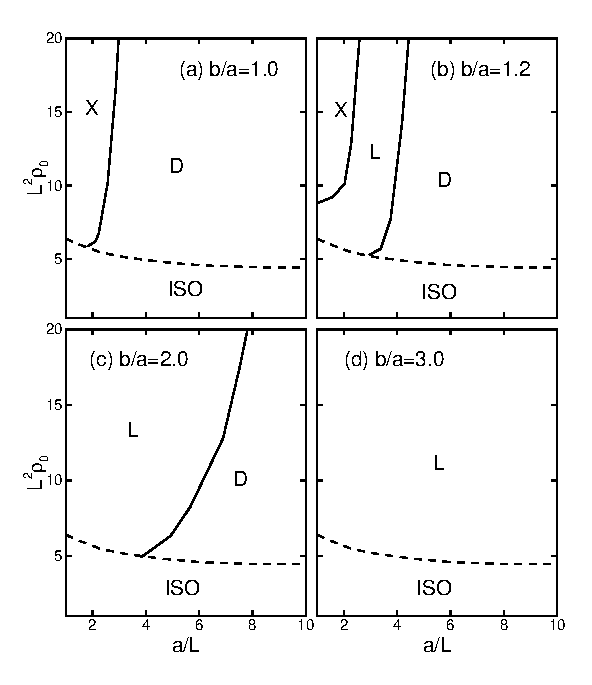
\includegraphics[width=0.7\textwidth]{./figs/ABCD.eps}
	\caption{Phase diagrams of the rectangular confined rod system from work \cite{yao} [PERMISSION?]. Here, $\rho_0 = N/a^2$ and the dashed line indicates a second-order phase transition.}
	\label{fig:phasediagram}
\end{figure}

\subsection{Orientational order}
Naturally, of great interest is a quantitative way to mark the whether a system is nematic of isotropic. That is, to mark when the higher symmetry of the isotropic phase is broken in the nematic phase. Qualitatively we describe this less symmetric nematic phase as having more order. The task then is to create an order parameter that vanishes to zero in the isotropic phase and approaches unity in the nematic phase.
For example, in a ferromagnetic system the magnetization is conveniently readily an appropriate order parameter. However, conjuring one for liquid crystals is less trivial.

We proceed with our derivation in three dimensions and then consider the two dimensional case. Naively one may opt for a directional average but since rods have a center of symmetry the average of $\bv{u}$ will cancel out. The next invariant is then the tensor
\begin{align}
	Q_{\alpha\beta} 
	= \frac{1}{N}\sum_i\left(u_\alpha^{(i)}u_\beta^{(i)} - \frac{1}{d}\delta_{\alpha\beta} \right),
\end{align}
in $d$ dimensions, where $\alpha$ and $\beta$ represent the Cartesian variables $x,y$ and $z$, $\delta_{\alpha\beta}$ is the Kroenecker delta, and the summation is a thermal average over a small but macroscopic volume. This $Q$-tensor has several useful properties:
\begin{itemize}
	\item It is symmetric since $u_\alpha^{(i)}u_\beta^{(i)} = 
	u_\beta^{(i)}u_\alpha^{(i)}$.\\
	
	\item It has zero trace:
	\begin{align*}
		\text{Tr}Q_{\alpha\beta} &= Q_{xx}+Q_{yy}+Q_{zz}\\
		&= \frac{1}{N}\sum_i\left[(u_x^{(i)})^2
		+ (u_y^{(i)})^2 + (u_z^{(i)})^2 - 1\right] \\
		&= 0
	\end{align*}
	since $\bv{u}$ is a unit vector.\\
	
	\item As the nematic approaches perfect alignment,
	\begin{align*}
		Q = \left(
		\begin{matrix}
		-1/3 & 0 & 0\\
		0 & -1/3 & 0\\
		0 & 0 & 2/3
		\end{matrix}
		\right),
	\end{align*}
	since $Q_{zz} = u_zu_z - 1/3 = 1 - 1/3 = 2/3$, then with $Q$ being traceless and the symmetry of $x$ and $y$, $Q_{xx}=Q_{yy}=-1/3$.\\
\end{itemize} 

A final and important property emerges, that $Q_{\alpha\beta} = 0$ in the isotropic phase. To see this we note in spherical coordinates
\begin{align*}
	u_x &= \sin\theta\cos\phi,\\
	u_y &= \sin\theta\sin\phi,\\
	u_z &= \cos\theta.
\end{align*}
We also introduce $f(\theta,\phi)$ as the probability of finding a molecule with angles $\theta$ and $\phi$ in the given region. Now, $Q_{\alpha\beta}$ may be equivalently expressed as
\begin{align*}
	Q_{\alpha\beta} = \int_0^{2\pi}d\phi \int_0^\pi \sin\theta d\theta f(\theta,\phi)\left( u_\alpha u_\beta - \frac{1}{3}\delta_{\alpha\beta}\right).
\end{align*}
In the isotropic phase $f(\theta,\phi) = 1/4\pi$. Thus, any $Q_{\alpha\beta}$ term of $x$ or $y$ is zeroed because of the periodic integral in $\phi$. This only leaves
\begin{align*}
	Q_{zz} &= \frac{1}{4\pi}\int_0^{2\pi}d\phi
	\int_0^\pi \sin\theta d\theta\left(\cos^2\theta - \frac{1}{3}\right)\\
	&= \frac{1}{6}\left(x^3 - x\right)\Big|_{-1}^1 = 0.\\
\end{align*}

Reducing to two dimensions is fairly straight forward. Our $Q$ tensor becomes
\begin{align}
	Q_{\alpha\beta} = \int_0^{2\pi}f(\theta)\left( 
	u_{\alpha}u_\beta - \frac{1}{2}\delta_{\alpha\beta} \right) d\theta,
\end{align}
where we now let $\theta$ describe the angle a rod makes with the $x$-axis. To generalize the expression for a given region centered on $(x,y)$, we simply have
\begin{align}
Q_{\alpha\beta}(x,y) = \int_0^{2\pi}f(x,y,\theta)\left( 
u_{\alpha}u_\beta - \frac{1}{2}\delta_{\alpha\beta} \right) d\theta,
\end{align}
with $f(x,y,\theta)$ now as the probability of a rod having orientation $\theta$ at the location $(x,y)$. We may concisely express $Q$ as the matrix
\begin{align}
	Q = \frac{1}{2}\left(
	\begin{matrix}
	S(x,y) & T(x,y)\\
	T(x,y) & -S(x,y).
	\end{matrix}
	\right)
\end{align}
Given $\bv{u} = (\cos\theta,\sin\theta)$, we define the elements
\begin{align}
	\nonumber
	S(x,y) = -2Q_{yy} = 2Q_{xx} &= 2\int_0^{2\pi} f(x,y,\theta)\left( \cos^2\theta - \frac{1}{2}\right) d\theta\\
	&= \int_0^{2\pi}
	f(x,y,\theta)\cos(2\theta)d\theta
\end{align}
and
\begin{align}
	\nonumber
	T(x,y) = 2Q_{xy} = 2Q_{yx} &= 2\int_0^{2\pi} f(x,y,\theta)\left( \cos\theta\sin\theta \right) d\theta\\
	&= \int_0^{2\pi}
	f(x,y,\theta)\sin(2\theta) d\theta.
\end{align}

Qualitatively, these elements describe the strength of alignment along the $x$ and $y$ axes, and their diagonals at $\theta=\pi/4$ and $3\pi/4$. $S(x,y)$ responds to alignment with the $x$ and $y$ axes, yielding $1$ for $x$-axis alignment and $-1$ for $y$-axis alignment. With $T(x,y)$, the response is $1$ for $\pi/4$-axis alignment and $-1$ for $3\pi/4$-axis alignment. We may also observe that both elements go to zero in isotropic phases. Finally, the eigenvalue of $Q$ pertains to the main order parameter measured from a local nematic director (Allen and Tildesly provide another reference, Zannoni 1979, on page 93 for eigenvalue and Q etc.),
\begin{align}
	\Lambda(x,y) \equiv \sqrt{S^2(x,y) + T^2(x,y)}.
	\label{e q:Lambda}
\end{align}

\begin{figure}
	\centering
	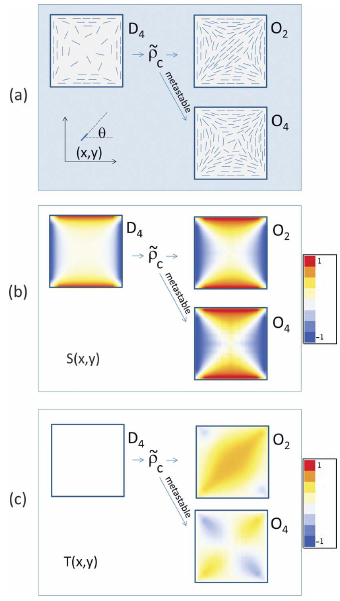
\includegraphics[height=0.86\textheight]{chen2013_ST.png}
	\caption{Stable D and metastable X solutions found in Ref.\ \cite{chen2013rods}. In their work the D state is labeled $O_2$ and the X state is $O_4$, with $D_4$ labeling the isotropic state. $\tilde{\rho}_c$ indicates a transition past the critical transition density. Order parameters $S$ and $T$ are also given. $T$ presents itself as an effective way to distinguish these two topologies.}
	\label{fig:TSmap}
\end{figure}

An intensity map of $T$ and $S$ on the stable diagonal D and metastable X solutions in Figure \ref{fig:TSmap} show how these parameters can be used to characterize different topologies.

Should we wish to determine a bulk nematic order parameter (which we do), we may take the mean values of $S(x,y)$ and $T(x,y)$,
\begin{align}
	\overline{S}(x,y) = \int_{-a/2}^{a/2} \int_{-a/2}^{a/2}\frac{S(x,y)}{a^2} dxdy,
\end{align}
\begin{align}
\overline{T}(x,y) = \int_{-a/2}^{a/2} \int_{-a/2}^{a/2}\frac{T(x,y)}{a^2} dxdy,
\end{align}
for box edge length $a$. In both cases, boundary effects will be annulled since rods order themselves parallel to wall edges \cite{wallordering}. A bulk order parameter 
\begin{align}
	\overline{\Lambda} \equiv \sqrt{\overline{S}^2 + \overline{T}^2}
\end{align}
may then be utilized to gauge if the whole system is in a nematic or isotropic state.

\begin{figure}
	\centering
	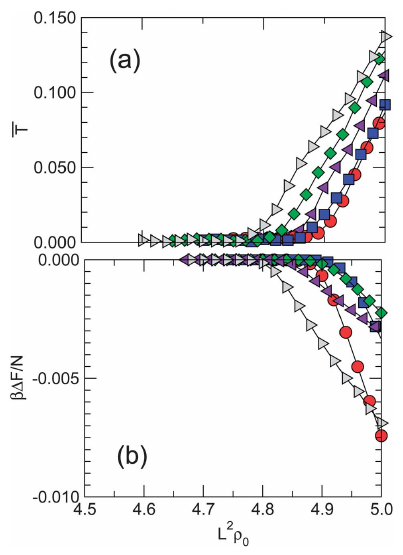
\includegraphics[height=0.55\textheight]{chen2013_Tavg}
	\caption{$\overline{T}$ as function...from \cite{chen2013rods}}
\end{figure}

\begin{figure}
	\centering
	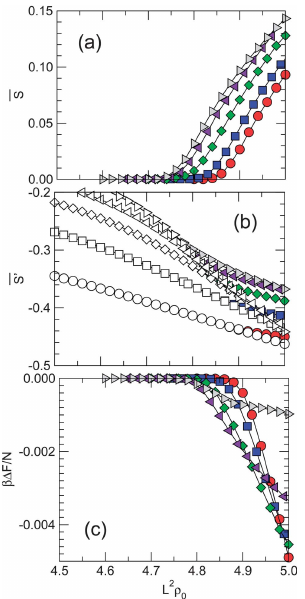
\includegraphics[height=0.8\textheight]{chen2013_Savg}
	\caption{$\overline{S}$ as function...\cite{chen2013rods}}
\end{figure}







%===========================

%===========================
\chapter{Computational Methods}
The Monte Carlo technique has been a widespread method for simulating liquid crystals and molecular dynamics at large. With credit generally awarded to John von Neumann, Stanislaw Ulam, and Nicholas Metropolis, the method was devised in the late 1940's as part of the Second World War effort by studying the diffusion of neutrons in fissionable material (\cite{allenbook} pg.\ 147). The principle is to treat a determinate mathematical problem with a probabilistic analogue and solve it by stochastic sampling. More specifically, we use the Metropolis Monte Carlo method published in 1953 by Metropolis \textit{et al.}\ \cite{metropolis1953}.

The method aims to explore the state space, while also tending towards states of higher statistical probability. We let $t$ count the number of ``Monte Carlo Steps'' (MCSs), where one MCS attempts $N$ random movements of molecules, either by iterating over the molecule list or randomly selecting $N$ molecules, though Ref.\ \cite{hastings1970} found iterating over the list equally valid with the benefit of being that bit simpler. We also let $\bv{\Gamma}(t)$ represent the system state at time step $t$, with $\bv{\Gamma}(0)$ being the initial state. In the case of our liquid crystal system of hard rods, a random rod movement would mean
\begin{align}
	\bv{r}_i(t+1) &= \bv{r}_i(t) + \delta\bv{r}\\
	\theta_i(t+1) &= \theta_i(t) + \delta\theta
	\label{eq:mcmoves}
\end{align}
for rod label $i$, and small spatial and angular displacements $\delta\bv{r}$ and $\delta\theta$. 
In the Metropolis algorithm, we must create a rule for the acceptance or rejection of a proposed move. We start by considering abstractly the state energy at time $t$, $E(t)$. The first condition in our rule is that if $E(t+1) < E(t)$, then this is energetically favourable and we accept the move (postponing the calculation of $E(t)$ for now). In the case of $E(t+1) > E(t)$ we do not flat out reject this. Instead we consider the Boltzmann factor, that is the probability of the system being in state $\bv{\Gamma}(t+1)$:
\begin{align}
	p_\Gamma(t+1) &= \frac{1}{Z}e^{-E(t+1)/k_BT}
\end{align}
with the canonical partition function $Z$. 
Further, we may compare the probability of this state with $\bv{\Gamma}(t)$ 
\begin{align}
	\nonumber
	\frac{p_\Gamma(t+1)}{p_\Gamma(t)} &= 
	\frac{e^{-E(t+1)/k_BT}}{e^{-E(t)/k_BT}}\\
	&=e^{-(E(t+1) - E(t))/k_BT} = e^{-\Delta E/k_BT}.
	\label{eq:pGamma}
\end{align}

We then base the decision of acceptance/rejection off this relative probability. To do so, a random number $\varepsilon$ is generated in the range $0\leq \varepsilon \leq 1$, and compared with the probability ratio $p_\Gamma(t+1)/p_\Gamma(t)$. The rule is to accept the proposed move if $\varepsilon < p_\Gamma(t+1)/p_\Gamma(t)$. 

\begin{figure}
	\centering
	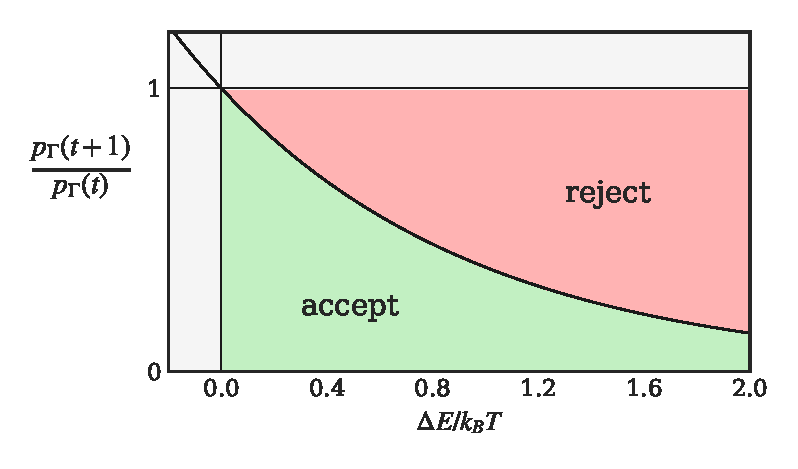
\includegraphics[width=0.8\textwidth]{mc_accrej.eps}
	\caption{Probability ratio of Eq.\ \ref{eq:pGamma} showing chances of acceptance or rejection upon generating $\varepsilon$ for a given $\Delta E$.}
	\label{fig:accrej}
\end{figure}

Figure \ref{fig:accrej} shows the chances of acceptance/rejection of a move for a given $\Delta E$. Moves that are energetically costly always have a finite chance of being accepted, though it is exponentially unlikely as $\Delta E$ increases. This feature is essential for the simulation to explore the phase space properly. Notice also that the acceptance approaches unity as $\Delta E \rightarrow 0$ as we expect.\\

In calculating $\Delta E/k_BT$, we needn't calculate the total system energies $E(t)$ and $E(t~+~1)$, rather since we only need their difference we simply calculate the energy change associated with the proposed move. As described in Ref.\ \cite{allenbook} pg.\ 156, the change in potential energy is calculated by summing over the interaction energies, $\epsilon_{ij}$, between our selected molecule $i$ and the other relevant molecules $j$,
\begin{align}
	\Delta E = \sum_j \epsilon_{ij}(t+1) - \sum_j \epsilon_{ij}(t).
\end{align}
This also has the advantage that interactions beyond a certain cutoff distance for both molecular positions, such as a mean field, cancel each other out.

Returning to our liquid crystal model of steric rods, the situation gains a simplification. Recall that the interaction potential of neighbouring molecules is approximated as a delta function: it is zero everywhere except for if there is an overlap at which point it is infinite. Thus, when a proposed move causes an overlap this results in $\Delta E = +\infty$, and conversely if the move grants no overlap, the system perceives no change in potential energy and $\Delta E = 0$. As these are the only two scenarios, we may circumnavigate the entire $\varepsilon$ generation and comparison phase, with an overlap having no probability of success and a non-overlap always being accepted.

It is up to the simulator to determine which magnitudes of $\delta\bv{r}$ and $\delta\theta$ from Eq.\ \ref{eq:mcmoves}  work best for their system. There is no theoretic solution for an optimal choice (\cite{allenbook} pg.\ 159). Generally, the smaller a degree of movement, the more likely a move is to be accepted. However, there is an inverse consequence in that the system generally explores the phase space more slowly. 
As briefly discussed in Allen \& Tildesly (\cite{allenbook} pg.\ 159), often simulators will choose a failure rate of around $0.5$, but a study by Ref.\  \cite{wood1959} found $0.9$ maximized the root-mean-square displacement of atoms as a function of computer time. Allen \& Tildesly soundly point out though, this study was carried out on a first generation computer (1959), with 32 hard spheres at a particular packing fraction, and there is no reason to believe that their optimum is universal, or even that root-mean-square displacement is always the desired metric for phase space exploration.


%===========================

%===========================
\chapter{Machine Learning with Neural Networks}
\begin{itemize}
	\item Let's think about the universal approximation theorem, proved by Hornik etal \cite{hornik1989multilayer}. A multilayer perceptron is a universal approximator of a function. Question though: can our problem be represented as a function? Let's think about a simple example of the input neurons being for $x$ and $y$ dimensions, and then the output being a singular neuron for $\cos(x)+\sin(y)$. That seems pretty sensible. I'm mostly concerned with how our input function is constructed so strangely. For example, if it's random whether $x$ or $y$ will be input to the first neuron, then this model breaks down.
	I do think the nature of the unreliability of this input vector means the approximation theorem doesn't apply. 
\end{itemize}

\section{FNN as a universal approximator}
There is a matter that cannot be ignored on this subject. The Universal Approximation Theorem for neural networks. Rigorously proved by Hornik, Stinchcombe, and White \cite{hornik1989multilayer}, the theorem's main points are:
\begin{itemize}
	\item Multilayer FNNs, even those with a single hidden layer, are universal approximators: they can approximate any continuous function to arbitrary accuracy.
	\item The above result is independent of choice of activation function so long as it is bounded and non-constant.
	\item Functions with finite support can be approximated exactly with a single hidden layer.
	\item Lack of success is due to insufficient number of hidden neurons \emph{or lack of a deterministic relationship between input and output}.
\end{itemize}
We emphasize the last point because it's believed this is the root cause of the failure of the FNN in learning the XTUD topologies. There is not consistency in what will appear in a given input node. For example, due to the randomness of the input loading, the same configuration may be loaded completely differently on separate instances.


\section{PCA detection of defects}
\subsection{Principal Component Analysis}
In this section we explore Principal Component Analysis (PCA) as a technique for detecting defect regions. PCA is a useful statistical method for transforming a dataset into a form that better distinguishes features in the data, and it may also be used as a dimension reduction tool on a dataset. It also falls into the category of unsupervised learning since it reveals features in the data without any label-directed goals. PCA is well-known, and we'll follow the explanation offered by Johnathan Shlens \cite{shlens2014pca}.

We let the $m\times n$ matrix $\bv{X}$ represent our dataset of $m$ observations on $n$ dimensions. The goal of PCA is to find the matrix $\bv{W}$ that \textit{best} transforms our dataset to a new set of orthogonal axes, or ``principal components'':
\begin{align*}
	\bv{Y} = \bv{X}\bv{W}.
\end{align*}
The $m\times n$ matrix $\bv{Y}$ then is our dataset projected onto this new set of axes. The \textit{best} axes of course are not arbitrary, but are such that they capture the maximal variance within the original dataset, with the variance monotonically decreasing with increasing axis index. In other words, the first PCA axis captures the largest variance, the second axis captures the next largest variance, and so on.
The column vectors $\bv{w_i}$ of $\bv{W}$ are in fact the unit vectors that describe the orientation of these new axes in the original $n$-dimensional space, and hence describe how each observation in $\bv{X}$ projects onto them.
The usefulness of this technique does rely on the assumption that a high variance along an axis indicates an important feature of the data, but this generally the case.

To begin, we note the covariance matrix of the $\bv{X}$ variables (adjusted to zero-mean to simplify calculations)
\begin{align*}
	\bv{C_X} = \frac{1}{m}\bv{X^TX}
\end{align*}
The diagonal elements of $\bv{C_X}$ are the variances of individual variables, and the off-diagonal elements are the covariances of different variables. We note that high covariances indicate a redundancy in our dataset, and we wish to minimize these.

We can now define a goal for optimizing $\bv{W}$: to diagonalize the covariance matrix $\bv{C_Y}$ of our transformed dataset. Such a matrix minimizes redundancy across variables and maximizes variance. There are multiple ways to diagonalize $\bv{C_Y}$, but PCA opts for a simple route by having PCA components form an orthonormal basis. 
To find $\bv{W}$ we perform an eigendecomposition on $\bv{C_Y}$ and find that the PCA components are in fact the eigenvectors of $\bv{C_X}$. We begin by writing $\bv{C_Y}$ in terms of $\bv{W}$:
\begin{align}
\nonumber	\bv{C_Y} &= \frac{1}{m}\bv{Y^TY}\\
\nonumber	&= \frac{1}{m}(\bv{W^TX^T})(\bv{XW})\\
\nonumber	&= \bv{W^T}\left(\frac{1}{m}\bv{X^TX}\right)\bv{W}\\
	&= \bv{W^TC_XW}.
\label{Eq:cycx}
\end{align}
We may draw on the property that any symmetric matrix $\bv{A}$ is diagonalizable, $\bv{A}=\bv{SDS^T}$, for diagonal eigenvalue matrix $\bv{D}$ and orthonormal eigenvector matrix $\bv{S}$. If we now define $\bv{W}$ as this matrix of eigenvectors for $\bv{C_X}$ (since $\bv{C_X}$ is symmetric), we have
\begin{align*}
	\bv{C_Y} &= \bv{W^T}(\bv{WDW^T})\bv{W}\\
	&= (\bv{W^TW})\bv{D}(\bv{W^TW})\\
	&= \bv{D},
\end{align*}
where we also use the orthonormality of $\bv{W}$. The eigenvalues, $\bv{\lambda}$, are also called the ``explained variance'' in this context. Their normalized values, $\lambda_i^* = \lambda_i/\sum\lambda_j$, or explained variance ratios, are used as a metric as to the importance of each axis, values close to $1$ indicate more significance and those closer to $0$ being less significant. Generally, one expects only some small number of dimensions to be significant and will see a noticeable drop in $\lambda^*$ indicating where component axes may be ignored.
We can verify that our conditions are met:
\begin{itemize}
	\item By Eq. \ref{Eq:cycx}, the $i$th diagonalized variance of $\bv{C_Y}$ is the variance of $\bv{X}$ along the $i$th principal component.
	\item $\bv{W}$ indeed diagonalizes $\bv{C_Y}$.
\end{itemize}

\subsection{PCA learning order parameters for phase transitions}
Recently, PCA has seen some fascinating use on condensed matter systems. In 2016, L.\ Wang (Ref.\ \cite{wang2016ising}), with a dataset of simulated Ising spin systems (each observation was an instance of a system and each spin location was a feature dimension of $\bv{X}$), PCA could locate phase transitions in both the standard Ising model, but also the conserved order parameter (COP) Ising model. In the standard model, reduction showed that only the first PCA component was significant for capturing the distinguishing information of the system. Indeed, the corresponding eigenvector $\bv{w_1}$ was simply a constant function, meaning that it was in fact the magnetization order parameter, and cluster analysis of the data along this component (although it was also visually evident) showed two clusters corresponding to the high and low temperature states. The author took things a step further with the COP model because each system had a net-zero magnetization, so the magnetization order parameter would not suffice and PCA would need to find other indicators of the phase transition. Championing this restriction, PCA found that four components were all that was necessary and together could form the structure factor indicative of the phase transition.

In 2018, authors R.B.\ Jadrich \textit{et al.}\ (Ref.\ \cite{jadrich2018offlattice}) applied PCA to detect phase transitions of multiple off-lattice systems, including the fluid-nematic transition of a liquid crystal system much like the one of focus here (although with ellipsoid molecules as opposed to rod-like). Their methods were similar to those just described, but instead of each observation being a whole system, they were smaller local samples centered on random probe molecules (e.g.\ the orientations of 20 nearest neighbours). Additionally, the off-lattice nature carried with it some ambiguity as to the structuring/ordering of the nearest neighbours that formed $\bv{X}$ dimensions. Using an intuitive distance-to-probe ordering, they found again only the first PCA component was needed to learn the transition, and that it modeled the classical order parameter used to locate the transition.

What is crucial to note here, and what is so exceptional about this method, is that, apart from the raw particle information (location, spin, orientation, etc.), it requires no additional information about each system such as Hamiltonians or interaction potentials. On top of this, PCA does not cluster observations in some black-box style, but discovers the precise order parameters that are classically used to indicate the phase change.

\subsection{PCA learning disclinations}
We now put forth the question: Can PCA use nearest neighbour information of our LC system to identify nematic vs.\ disclination/defect states of the variety shown in Fig, or beyond that which \textit{type} of defect?
The following discusses this question, with results on the endeavor presented in Sec.\ \ref{Results}.

The results of Ref.\ \cite{jadrich2018offlattice} are certainly encouraging, though their objective was somewhat different. PCA detected a long-range angular correlation appeared signaling the nematic phase, and for this they used every \nth{10} nearest neighbour. Here we are concerned with detailed local features. In theory, the nematic vs.\ non-nematic states should be differentiable. For a given probe $i$ (either a rod or a point in space), we may construct a feature vector $f_i = [x_1^{(i)},x_2^{(i)},\cdots,x_{nn}^{(i)}]$ of some physical quantity $x$. Rod orientation relative to the probe rod $\theta_{ij}$ or, to account for the rod symmetry, the transformed $\cos(2\theta_{ij})$ may be sufficient, but the probe rod orientation is highly variable within a characteristic defect orientation, so defects may appear significantly different in their feature vectors. A counter to this would to take neighbouring rod orientations with respect to a local nematic director $\alpha$ isntead. 

A random ordering of neighbours may work in detecting nematic vs.\ defect states, but would not be expected to work for the more detailed defect type detection. In a perfectly shaped defect, a maximal $\theta_{\alpha j}$ or frequency of certain angles may signal a defect type, but the Monte Carlo defect samples would have too much overlap/similarity for a randomly ordered feature vector. Thus, in the same way that humans visually identify winding numbers, a feature vector that is ordered by a clockwise procession around the defect center should be a more effective approach.



\begin{figure*}[!t]
	\centering
	\begin{minipage}[t]{0.25\textwidth}
		\centering
		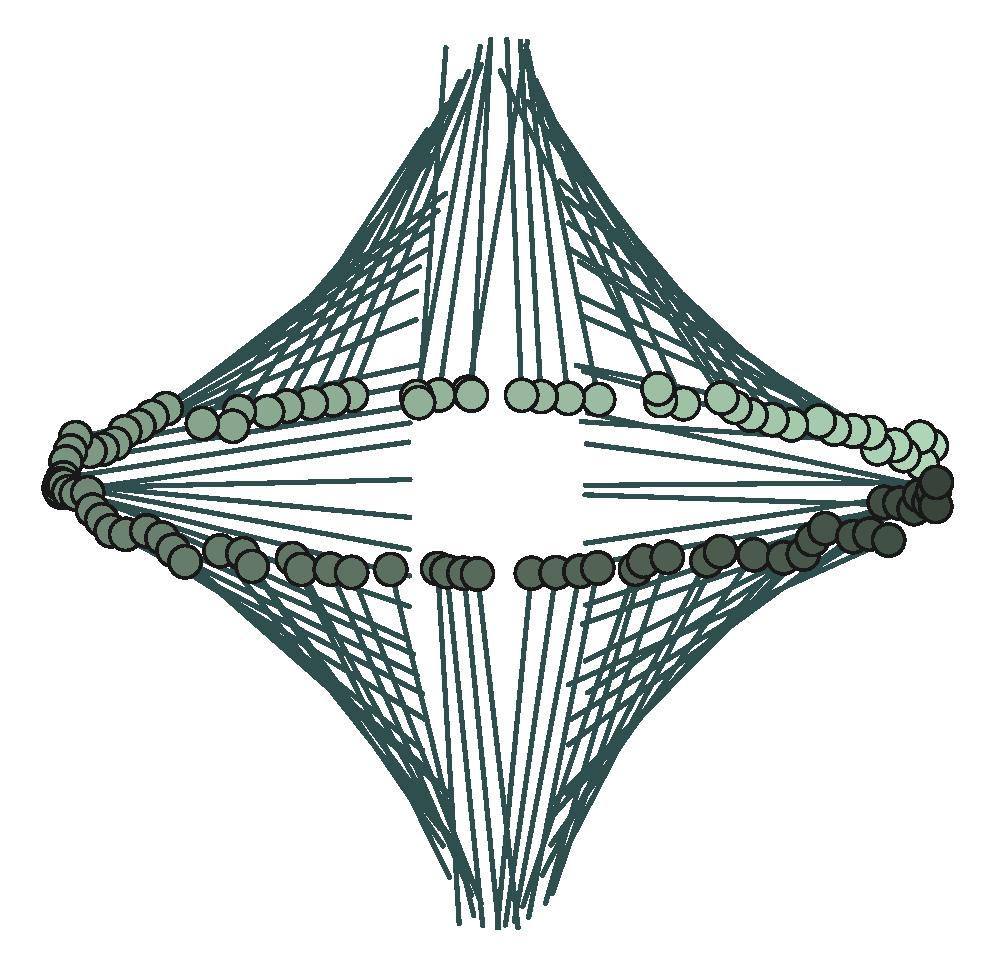
\includegraphics[width=0.9\columnwidth]{./figs/minusone_reruns_0_alt.eps}\\
		(a)\\ \vspace{0.5cm}
		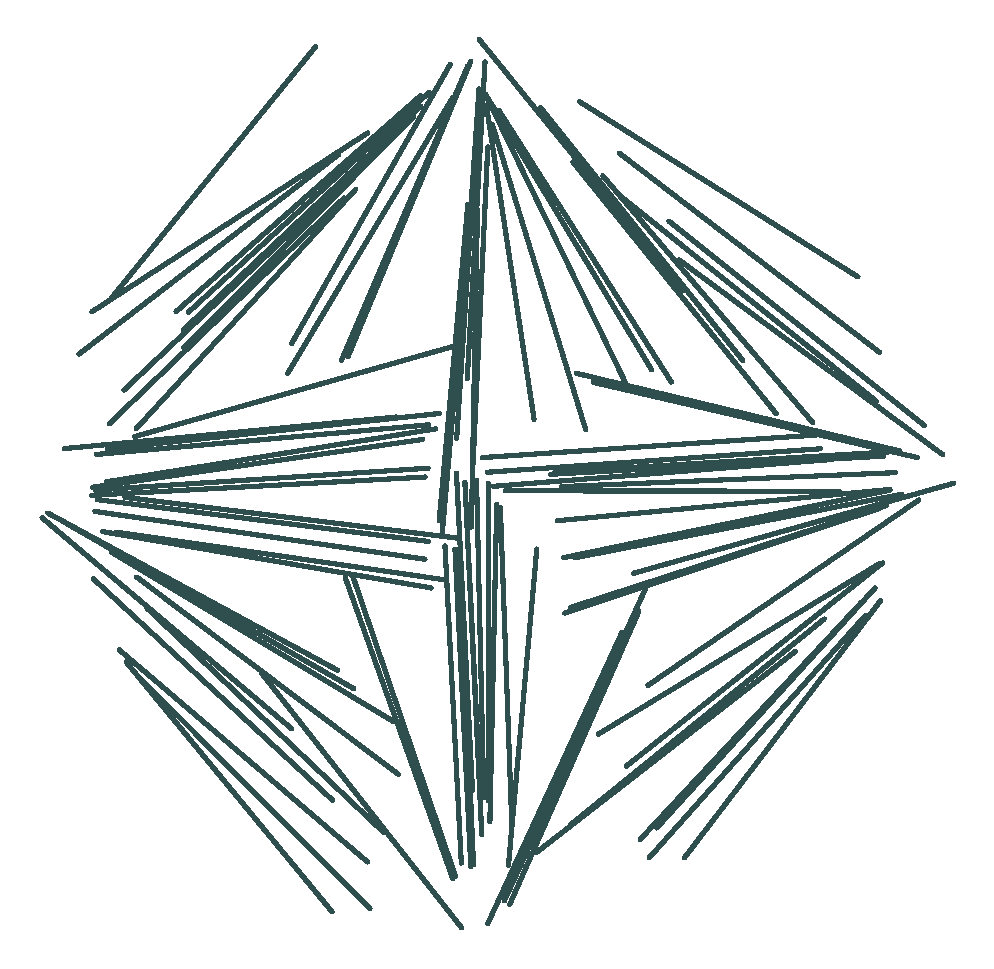
\includegraphics[width=0.9\columnwidth]{./figs/minusone_reruns_1_alt.eps}\\
		(e)
	\end{minipage}%
	\begin{minipage}[t]{0.25\textwidth}
		\centering
		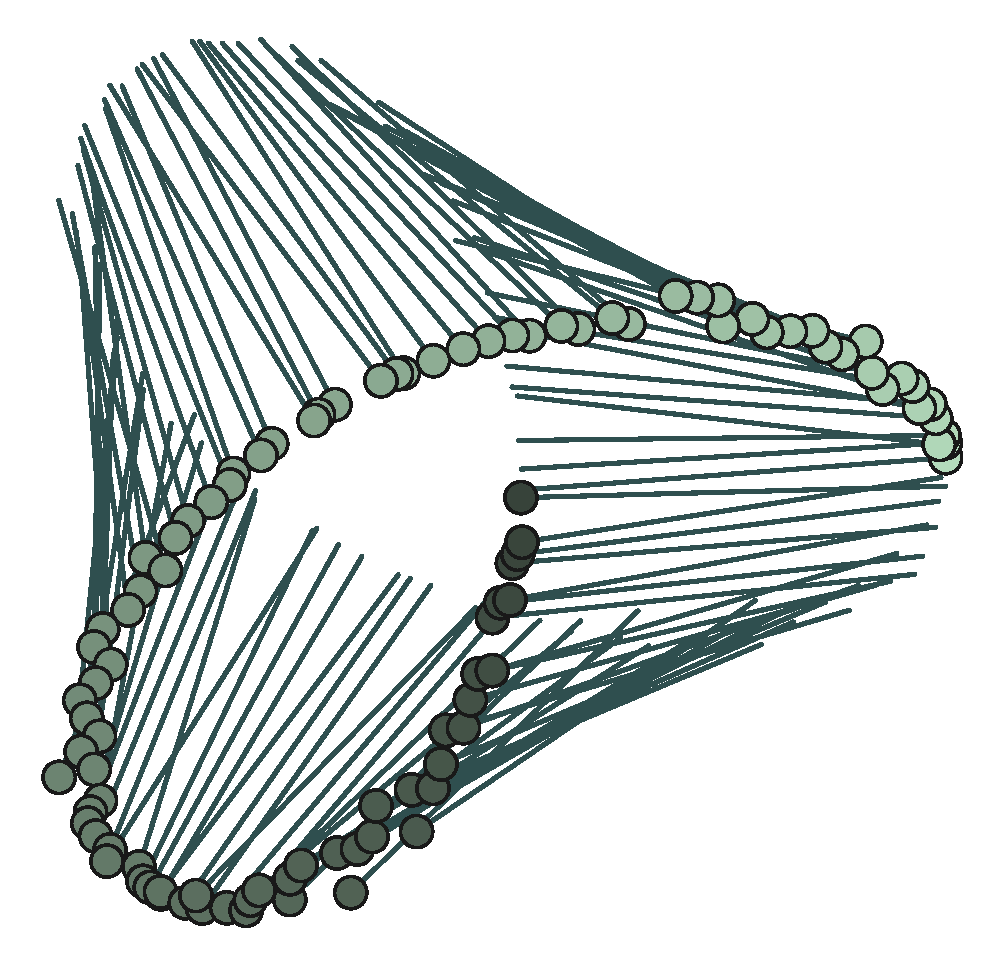
\includegraphics[width=0.9\columnwidth]{./figs/minushalf_reruns_0.eps}\\
		(b)\\ \vspace{0.5cm}
		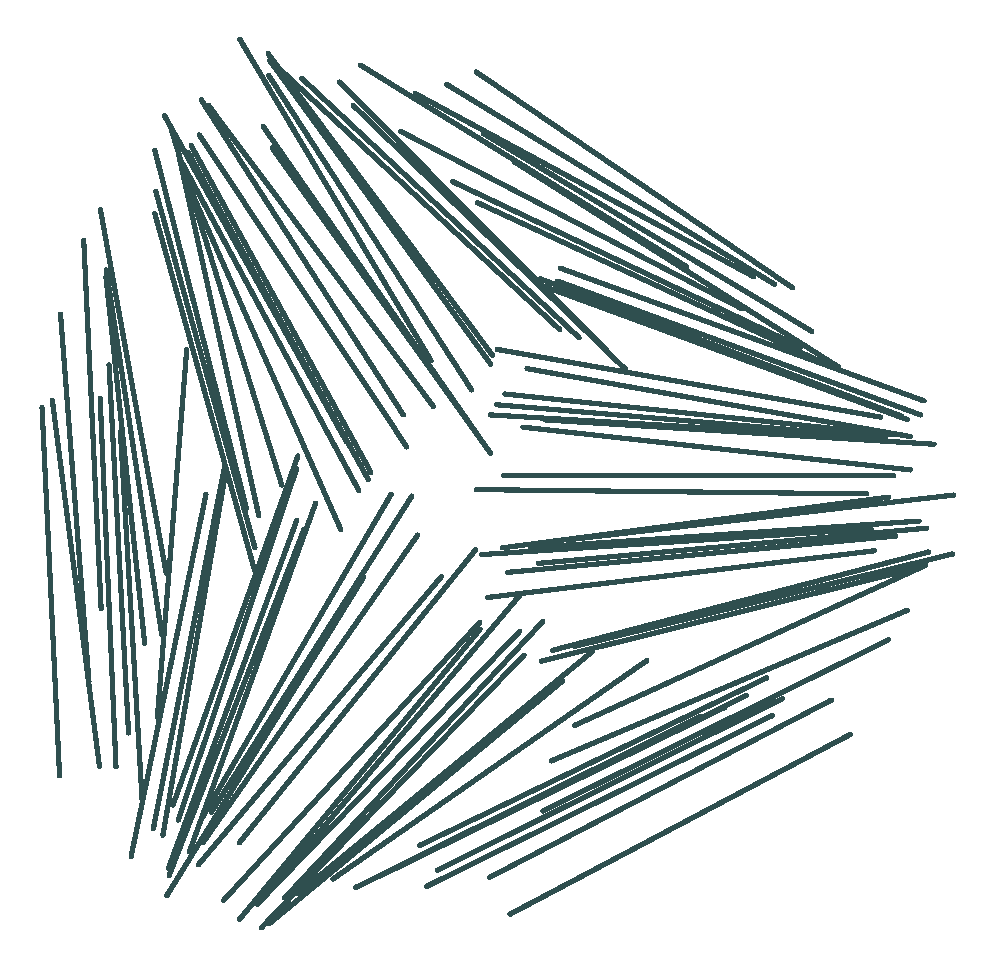
\includegraphics[width=0.9\columnwidth]{./figs/minushalf_reruns_1.eps}\\
		(f)
	\end{minipage}%
	\begin{minipage}[t]{0.25\textwidth}
		\centering
		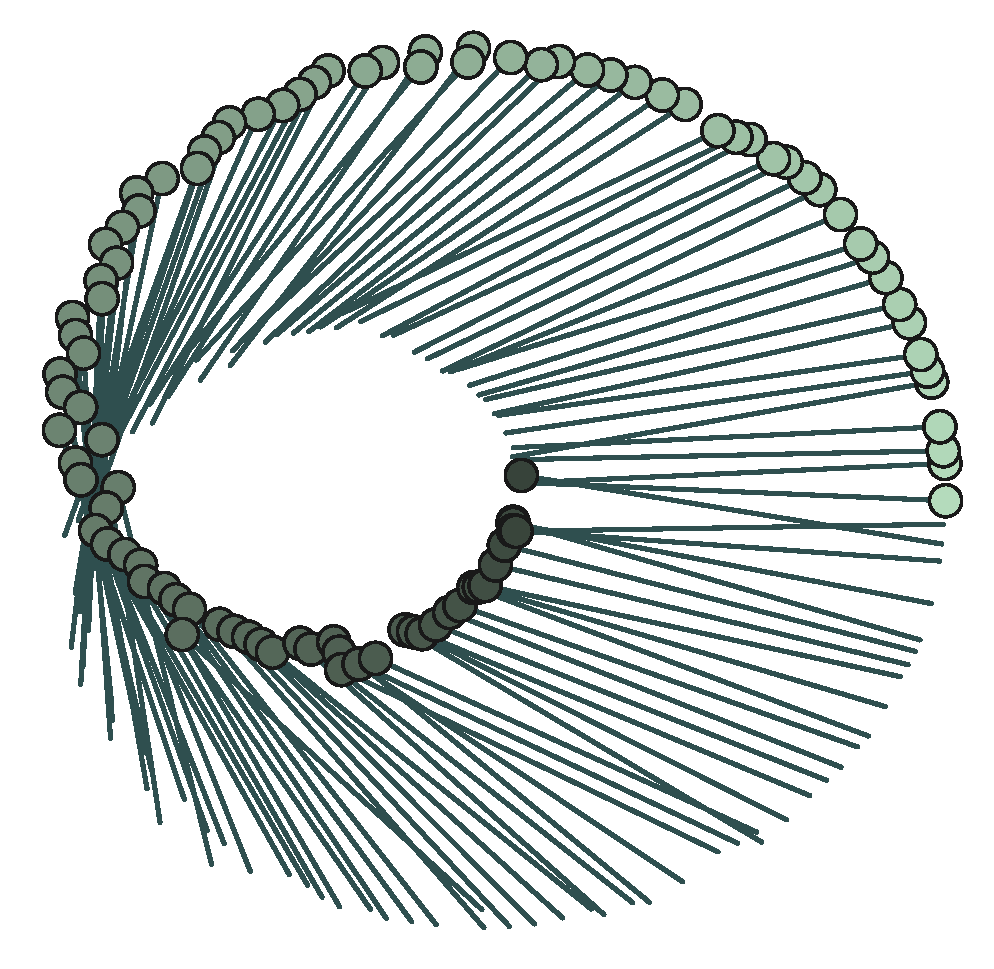
\includegraphics[width=0.9\columnwidth]{./figs/plushalf_reruns_0.eps}\\
		(c)\\ \vspace{0.5cm}
		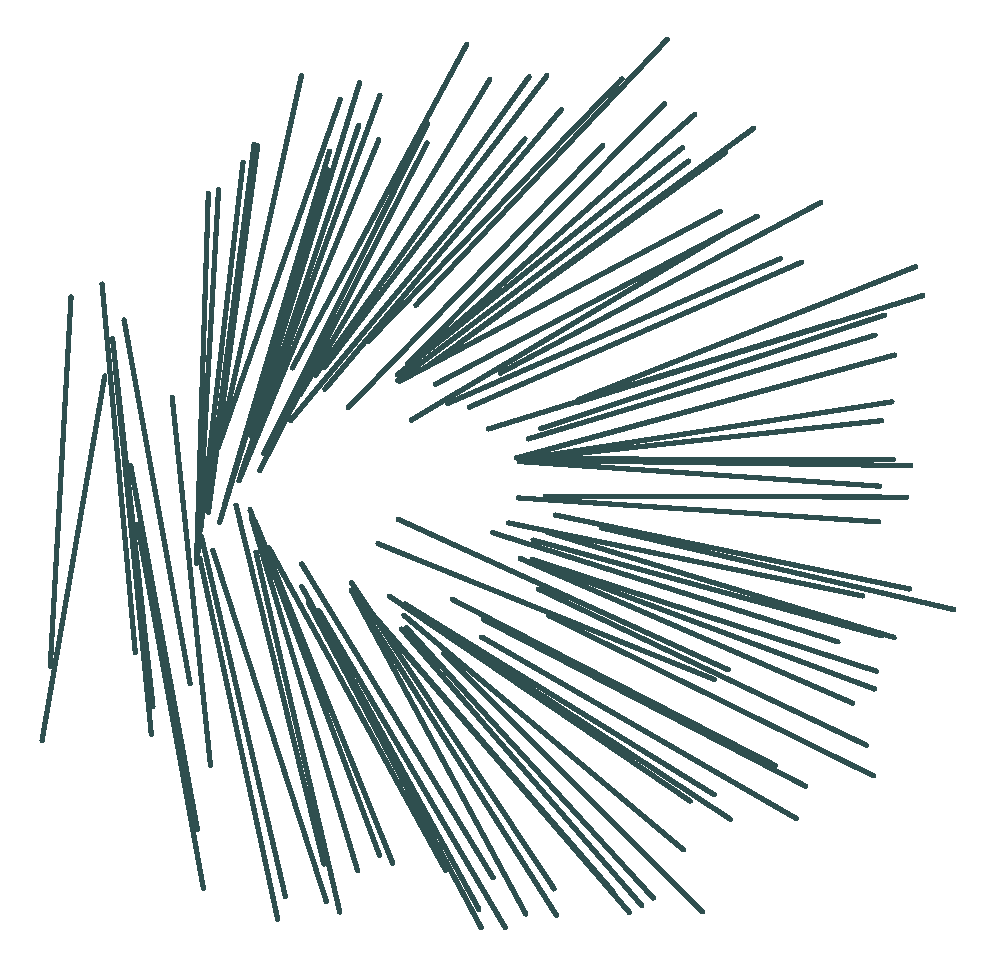
\includegraphics[width=0.9\columnwidth]{./figs/plushalf_reruns_1.eps}\\
		(g)
	\end{minipage}%
	\begin{minipage}[t]{0.25\textwidth}
		\centering
		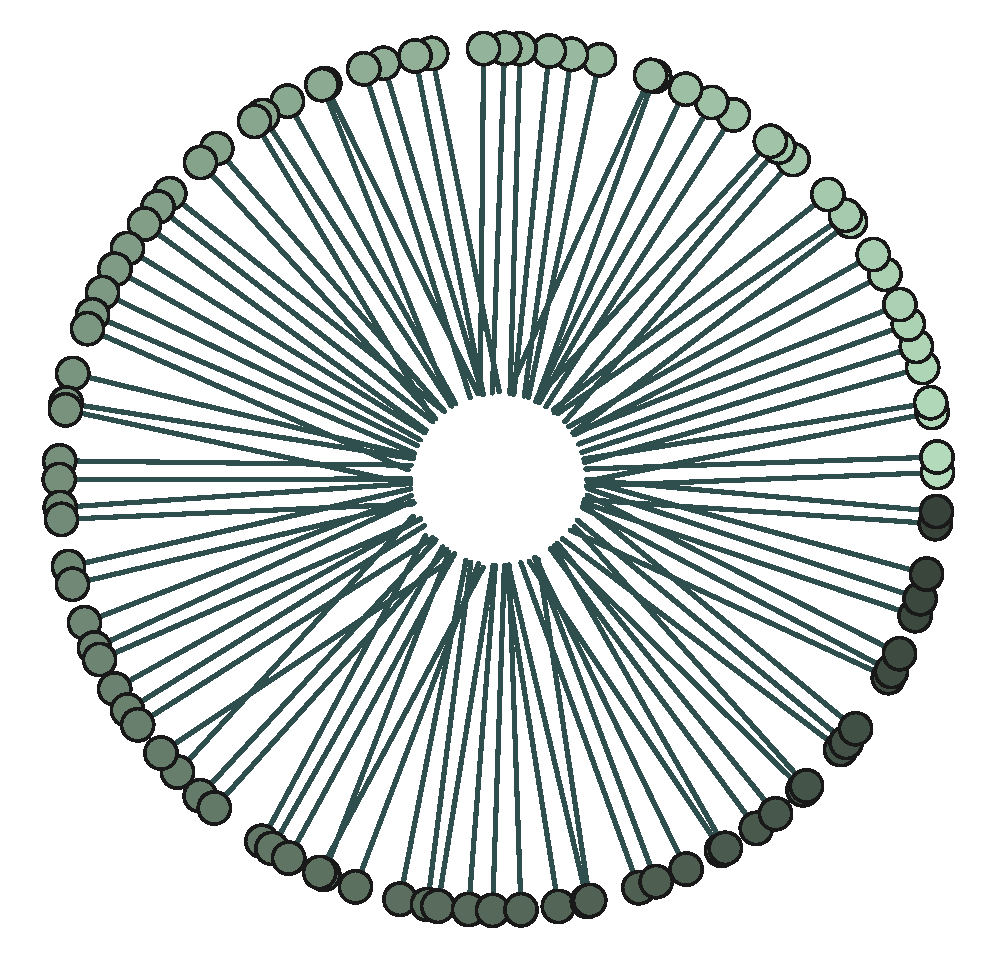
\includegraphics[width=0.9\columnwidth]{./figs/plusone_reruns_0.eps}\\
		(d)\\ \vspace{0.5cm}
		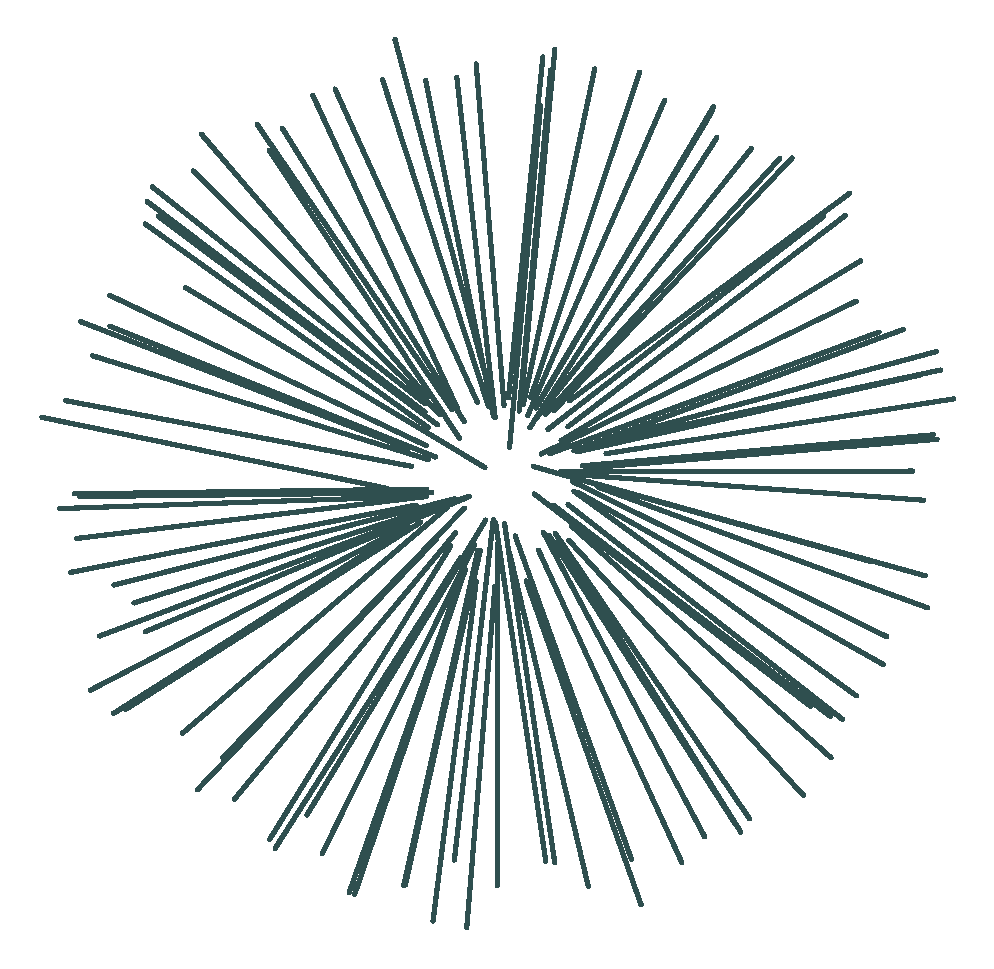
\includegraphics[width=0.9\columnwidth]{./figs/plusone_reruns_1.eps}\\
		(h)
	\end{minipage}%
	\caption{(a)-(d) Examples of initialized disclinations with winding numbers $-1$, $-1/2$, $+1/2$, and $+1$ respectively, as a visual aid for understanding the procession around the defect center. In proceeding clockwise around a defect, winding polarity indicates the direction of rotation about the rod axis, and magnitude indicates how many rotations about this axis. Coloured dots are included as a visual aid. (e)-(h) Below, uncrossed samples of the above disclinations. Such uncrossed samples made up the defect PCA dataset.
	}
	\label{FIG:defects_pure}
\end{figure*}

We adopt an approach where we first identify a nematic director $\alpha$ from neighbours. We use a discretized version of the method outlined in Section \ref{Order param} that produces the $Q$-matrix in equation \ref{eq:Qmat}:
\begin{align*}
	Q_{nn} = \frac{1}{2}\left(
	\begin{matrix}
	S_{nn}(x,y) & T_{nn}(x,y)\\
	T_{nn}(x,y) & -S_{nn}(x,y).
	\end{matrix}
	\right)
\end{align*}
where $S_{nn}$ and $T_{nn}$ are averaged over neighbours,
\begin{align*}
	S_{nn} &= \frac{1}{N_{nn}}\sum_i \cos(2\theta_i)\\
	T_{nn} &= \frac{1}{N_{nn}}\sum_i \sin(2\theta_i)
\end{align*} 












%===========================

%===========================
\chapter{Results}
\label{Results}
%\usepackage[pdftex]{graphicx} % For including graphics N.B. pdftex graphics 

\begin{itemize}
	\item Chen 2015 (Theory of wormlike polymers) discusses the NI transition density
\end{itemize}

The use of neural networks as a tool in condensed matter research has seen a growth in popularity. One of the marvels and advantages of this technique is how little statistical-physics information (energies, order parameters, etc.) is needed for the classification of states or the pinpointing of critical physical parameters.
Even relatively simple neural network models can learn phase-transition temperatures, order parameters, and quantum-state tomography, from the information of a simple feature such as position coordinates in an off-lattice model or the location and value of spins in an Ising model. This could all be done without any knowledge of the original Hamiltonian or interaction potential energies \cite{torlaiboltzmann,carras,wei,wetzel,torlai,morningstar,beach}.


\begin{figure*}[!t]
	\centering
	\begin{minipage}[t]{0.25\textwidth}
		\centering
		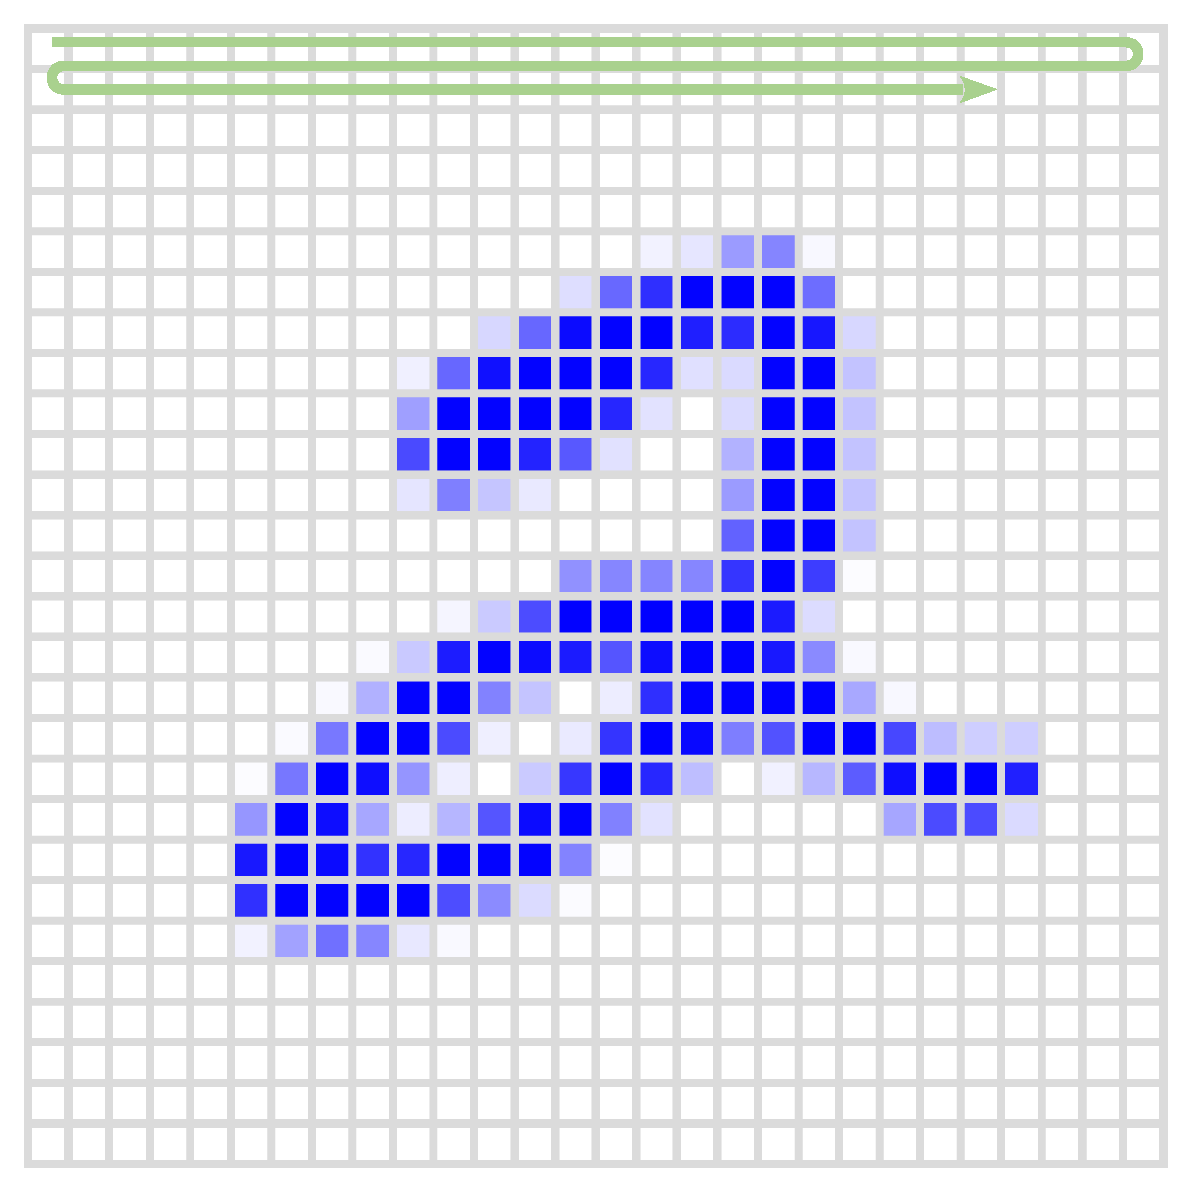
\includegraphics[width=0.9\columnwidth]{./figs/FIG1A.eps}\\
		(a)\\ \vspace{0.5cm}
		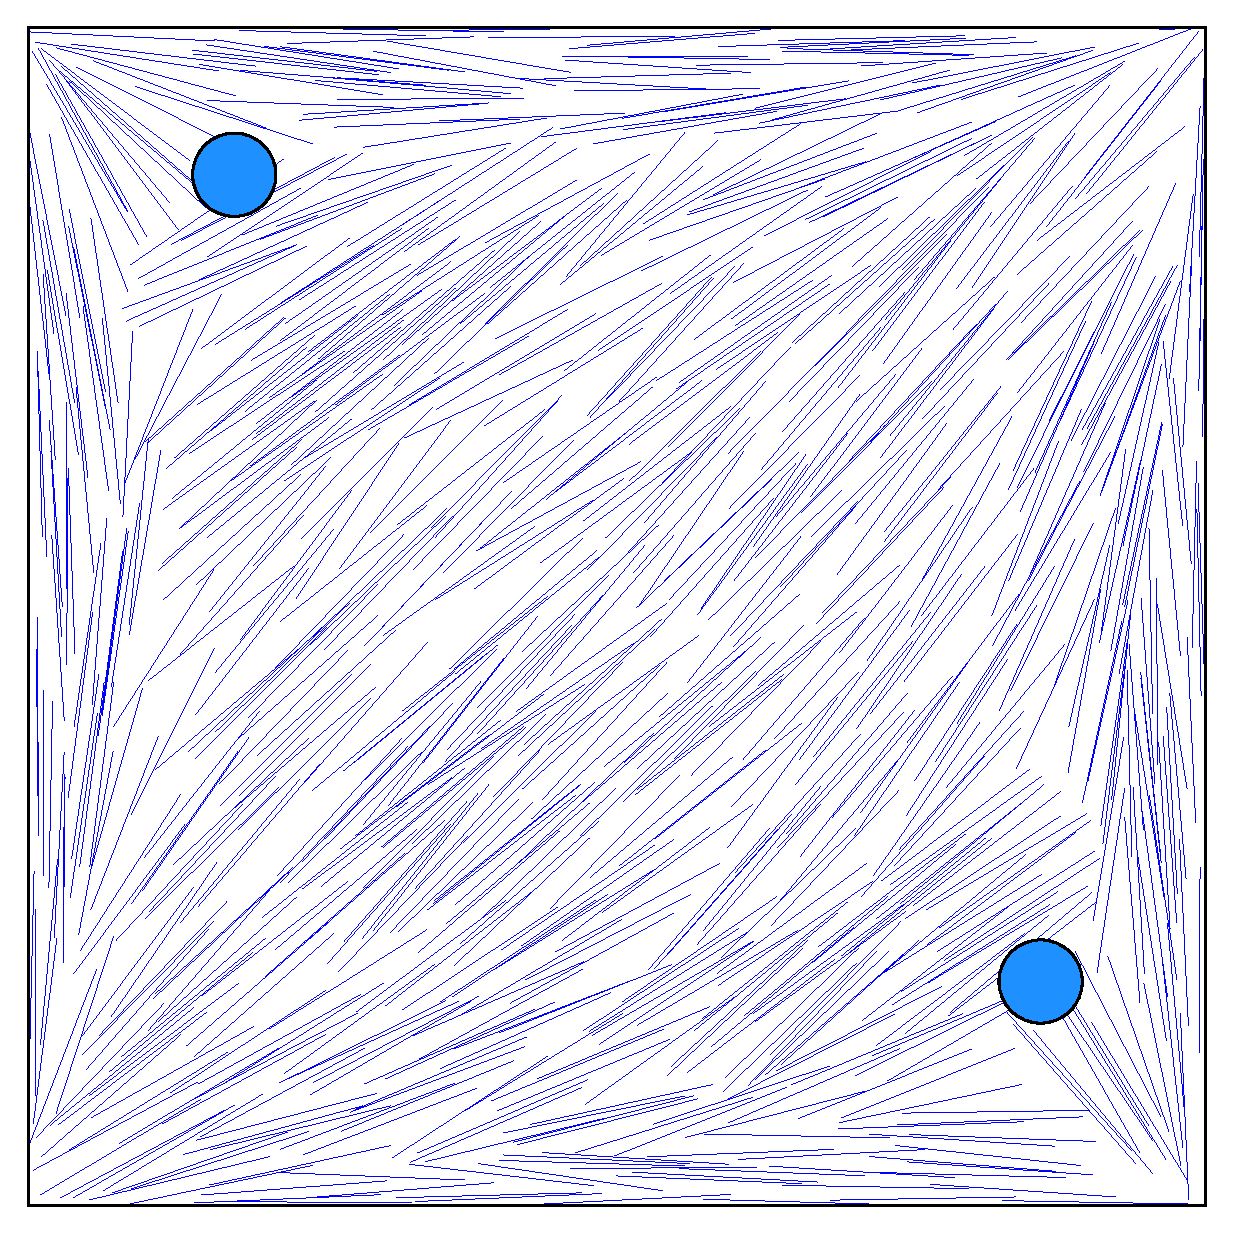
\includegraphics[width=0.9\columnwidth]{./figs/FIG1E.eps}\\
		(e)
	\end{minipage}%
	\begin{minipage}[t]{0.25\textwidth}
		\centering
		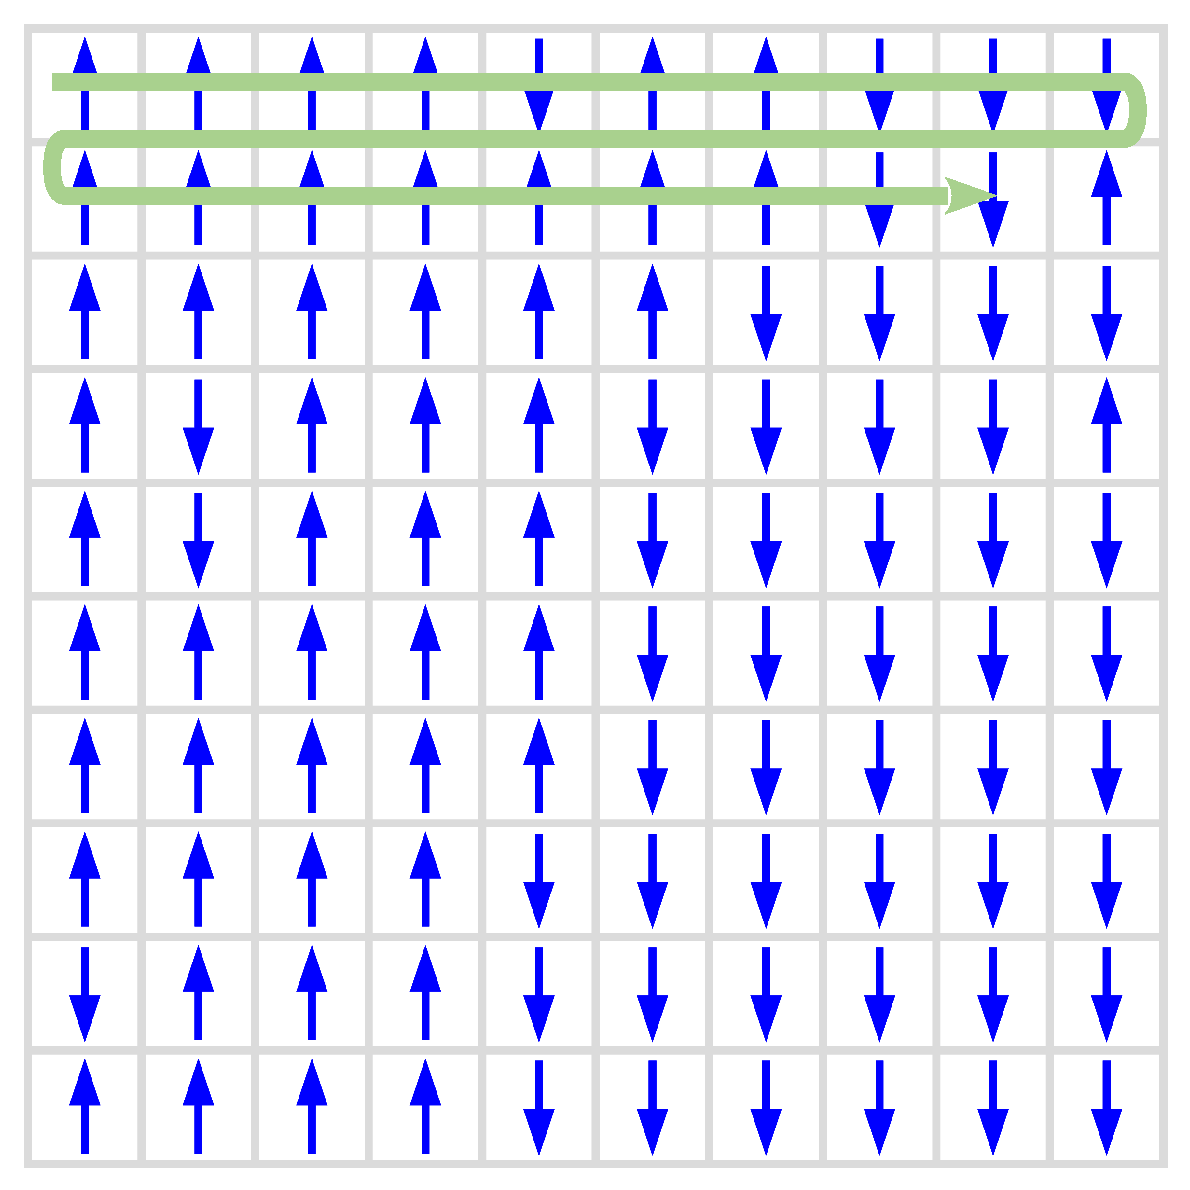
\includegraphics[width=0.9\columnwidth]{./figs/FIG1B.eps}\\
		(b)\\ \vspace{0.5cm}
		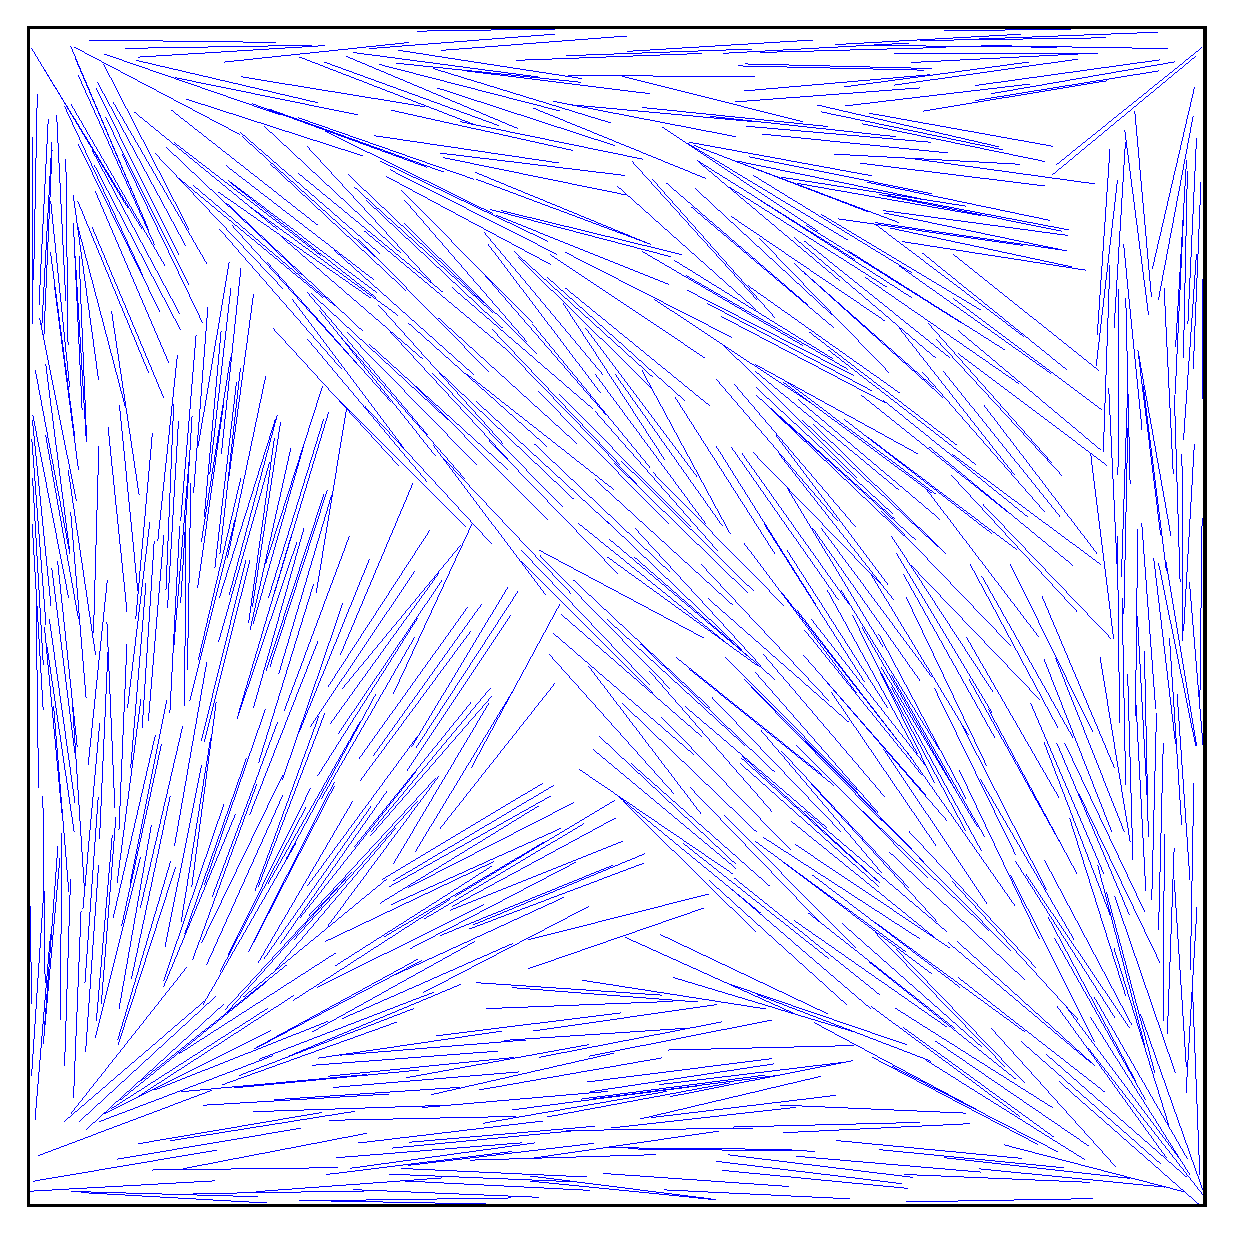
\includegraphics[width=0.9\columnwidth]{./figs/FIG1F.eps}\\
		(f)
	\end{minipage}%
	\begin{minipage}[t]{0.25\textwidth}
		\centering
		
\includegraphics[width=0.9\columnwidth]{./figs/FIG1C.eps}\\
		(c)\\ \vspace{0.5cm}
		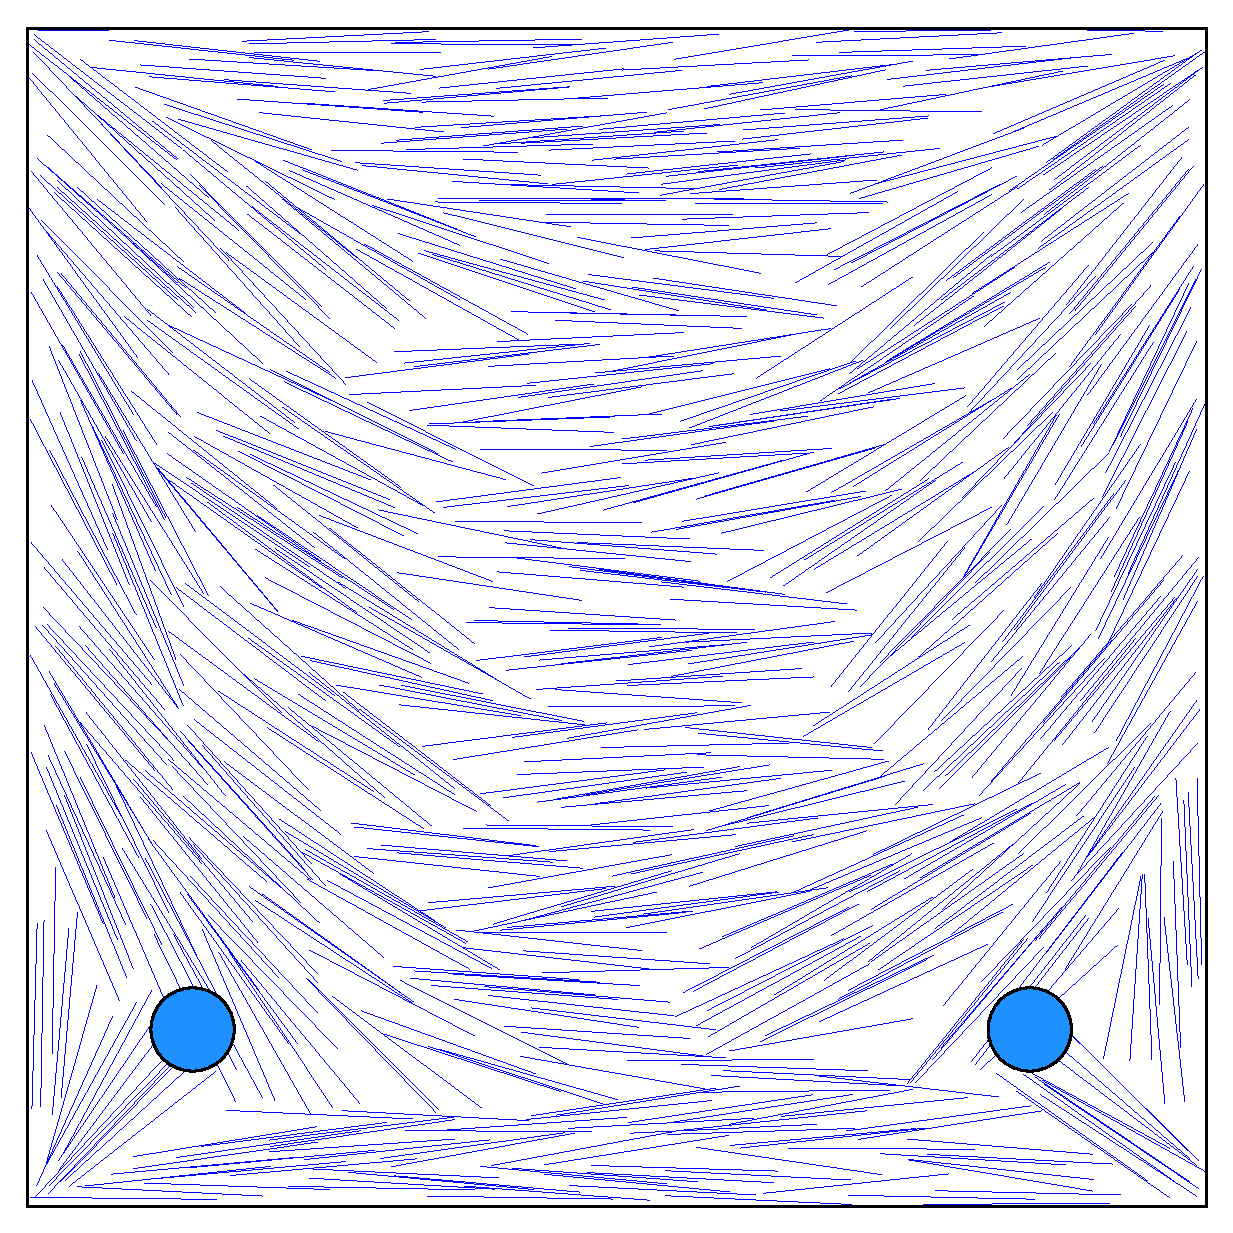
\includegraphics[width=0.9\columnwidth]{./figs/FIG1G.eps}\\
		(g)
	\end{minipage}%
	\begin{minipage}[t]{0.25\textwidth}
		\centering
		
\includegraphics[width=0.9\columnwidth]{./figs/FIG1D.eps}\\
		(d)\\ \vspace{0.5cm}
		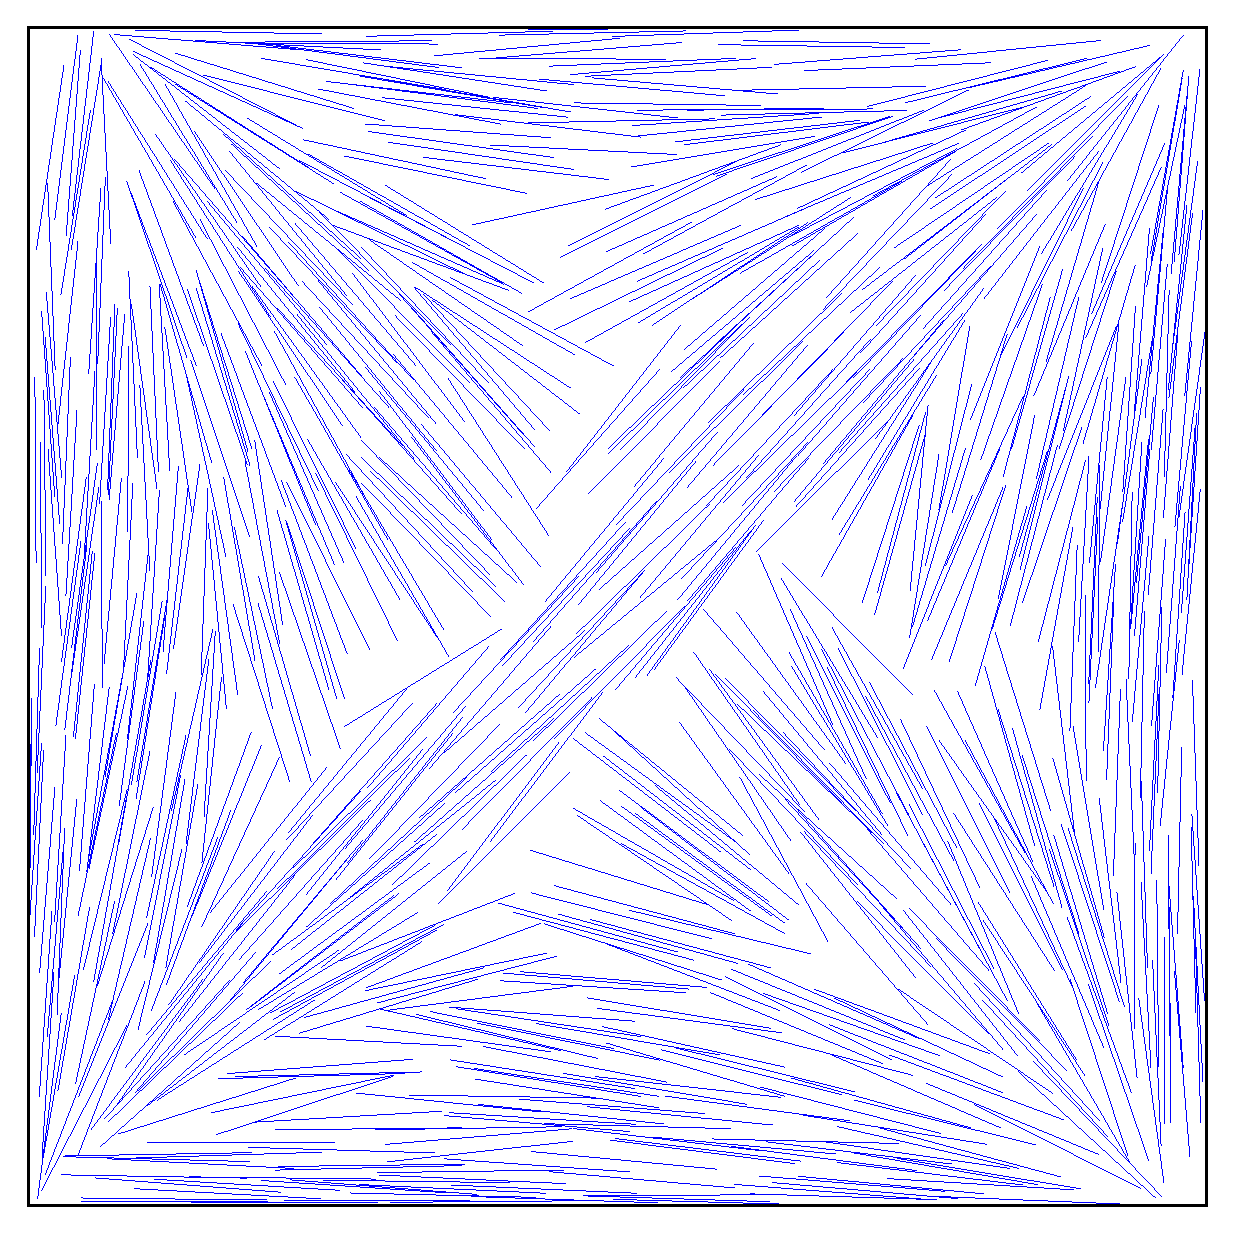
\includegraphics[width=0.9\columnwidth]{./figs/FIG1H.eps}\\
		(h)
	\end{minipage}%
	\caption{(a)-(d) Illustration of a two-dimensional hand-written image, Ising model, nematic state, and coordinates for a rodlike molecule,
		as well as (e)-(h) example configurations of different defect states generated from
		Monte Carlo simulations for a
		confined rodlike nematic fluid.
		The parameters used to generate these example configurations are $[N,L/a]=[784,6.32]$.
		The defect state in (e) has a diagonal (D) pattern, and
		the nematic textures in (f)-(h) resemble the tilted letter T, letter U, and letter X. 
	}
	\label{FIG1}
\end{figure*}

One of the simplest neural networks is the feedforward neural network (FNN). A powerful tool, FNNs are able to accomplish a variety of image recognition tasks \cite{schmidhuber_deep}, a frequent benchmark test being the MNIST hand-written digit data set \cite{mnistset}. Figure \ref{FIG1}(a) shows one such digit from the MNIST set. Increasing the size and depth of a network boosts its ability to learn more complex patterns and features contained in images and then recognize these learned patterns in a new image.
An extension of the FNN, the convoluted neural network (CNN), has the network structure organized in such a way that local features of a pattern are dissected \cite{cnnmnist}.
CNNs have thus been a natural choice for condensed matter research, in particular problems on lattices such as the Ising model \cite{carras}, the XY model \cite{beach}, correlated fermions \cite{broecker,chng}, and other quantum systems.

In condensed matter physics we often deal with ordered states, where
certain physical features display spatial correlations in long range. Two typical examples are shown in Fig.\ \ref{FIG1}. In the ferromagnetic state, within an ordered domain spins align in one direction, as illustrated in Fig \ref{FIG1}(b). In the nematic liquid crystal state, within an ordered domain molecular directions are all aligned towards a common angle [Fig \ref{FIG1}(c)].
The images produced in these examples can come from computer simulations, e.g. Monte Carlo simulations (see Appendix A for the current liquid-crystal system).
%%FNNs and CNNs are effective tools for identification of the disorder-to-ferromagnetic transition in the Ising model \cite{carras} and the isotropic-nemetic transition in the liquid crystal model [see Appendix B], when trained to recognize these different states.
Here, an ``image'' used for network learning is not a graphic image in the conventional sense. Rather, it is represented by the system configuration data containing physical features of each molecule (values of spins, angles specifying the orientations, etc).

These ordered states, on the other hand, sometimes have topological defects in their substantially ordered background. Different patterns can be characterized by different ways in which the local order parameters around the defects couple with the locations of the defects. Developing a characterization procedure to categorize these defects is a challenging task. A neural network (NN), then, becomes an ideal tool to identify these topological defects.
%In studying the Ising model with a neural network \hl{[IS THIS the paper for defect** We need to cite the defect paper here***]} \cite{carras}, an FNN was trained to recognize both high temperature (isotropic) states and low temperature (ferromagnetic) states. To read a given instance the neural net was given an ordered list of spins, from top-left to bottom-right. From this information alone the NN could learn the phase transition temperature, that is, it learned when contiguous regions were present or not.
%It would seem, then, the procedure is clear: a network with straightforward feeding of configurations through the input layer should enable the identification of defects in ordered states.
In studying the Kosterlitz-Thouless transition of the XY model \cite{beach}, a multilayered  network was trained on raw orientational configurations to learn the vortex unbinding that marks the transition. Accomplishing this requires the NN to understand topological features not too unlike the liquid crystal topologies in Fig.\ \ref{FIG1}(e)-(h). It would seem then that feeding the liquid crystal configurational data in a similar fashion should enable the identification of defects in ordered states.

However, we show here that such network structures are not readily appropriate for studying defect types of {\emph{off-lattice}} problems, such as the liquid-crystal defects shown in Fig.\ \ref{FIG1}((e)-(h)).
A typical configuration file generated from the computer simulations has a single-line data structure $[l,x_l,y_l,\theta_l]$ for a given molecule, where $l$ is the label of a molecule, and $[x_l,y_l, \theta_l]$ specify its $x$- and $y$- location coordinates and angular orientation [see Fig \ref{FIG1}(d)].
Because the molecules are allowed to randomly move in space, the label of a molecule, $l$, has no relationship at all with the spatial coordinates [see Fig \ref{FIG1}(c)].
This can be contrasted with a simulated data file produced by a lattice-model. In such a case, positional information is already embedded in the order in which molecules are labeled (one naturally reads the data in the same order every time), as demonstrated by the arrow in Fig.\ \ref{FIG1}(b).
An NN that attempts to capture position-correlated patterns is thus implicitly aided from this direct mapping of physical position to the ordering of data in a lattice model.

Hence, we must solve how to capture the main features in a topological-defect state when the correlation between defect positions and the physical properties around them is the vital property. In this paper we discuss different ways of incorporating existing NNs for this purpose. As it turns out, an FNN (and conceivably a CNN) finds correlation between the order of appearance of data in the input and the physical features to be correlated. Hence, FNNs and CNNs  can identify defect states resultant from the Ising model since the ordering of data already represents the spin positions. On the other hand, in an off-lattice model, $l$ has no correlation with  $[x_l,y_l, \theta_l]$. Even if we use $x_l, y_l$ as an input together with $\theta_l$, an FNN cannot find the correlation between $l$ and the input features $[x_l,y_l, \theta_l]$. This is discussed in Sect. \ref{FNN}.

Can we re-connect a relationship between $l$ and $x_l, y_l$ that can be easily used by an FNN for an off-lattice dataset? In Sect.
\ref{FNN} we develop and discuss a coarse-graining method which cuts the original simulation box into $m\times m$ equally sized cells where $m=1,2,4,8..$. The NN input is then ordered by cell index $M$, with the information inside each cell unordered. By such means, it is as though the system is approximated to a lattice form, with increasing accuracy as the cells become smaller and more numerous. An FNN can then begin to correlate physical features with position and identify topological defects with appropriate cell size.

However, we present another more general method, using a recurrent neural network (RNN), that avoids the need for any presorting.
The RNN is a neural network specialized in correlating sequential information (e.g.\ analyzing a time series of images \cite{rnnvideo}, or predicting upcoming words in a sentence based on previous words \cite{rnnwords1,rnnwords2}). In Sect. \ref{RNN}, we propose a scheme to feed
$x$, $y$, and $\theta$ data sequentially, akin to three time sequenced images, which enables the RNN to correlate these three features. Turning temporal correlation to spatial correlation, an RNN can efficiently identify topological defects in the original raw data, without any of the coarse-graining or presorting needed for the FNN.

We selected the topological defects appearing in the system of $N$ rodlike molecules confined by a square boundary in two dimensions (2D) as a
vehicle to deliver some of the concepts in this paper. This system has been the focus of recent theoretical and experimental studies due to its practical relevance \cite{Galanis2006,Mulder2011,Lewis2014,Cortes2017} and interesting theoretical aspects \cite{Tsakonas2007,Luo2012,chen2013rods,Mulder2015,Lewis2014}.
% above sources pulled from Yao fig 6 (earlier version)
In Ref. \cite{yao}, this system was studied in-depth, producing an ensemble of stable and metstable states. Our aim here is not a detailed study of this particular liquid crystal system, which has been done in the above listed references.
Rather, the system gives us the four major defect states, D, T, U, and X, shown in Fig.\ \ref{FIG1}(e)-(h), which we can use as examples in our machine learning study. The computer simulation procedure, as well as the system's isotropic-nematic transition properties, are explained in Appendices \ref{MC} and \ref{IN}.

Returning to the classic example of identifying hand-written numerical digits from 0 to 9, we make a comparison between the darkened pixels in this case with the topological defects in our confined liquid crystal system. In a sense, what a neural network looks for is the feature correlation of the spatial position of the darkened pixels in these images. In Appendix \ref{AppMNIST}, we re-enforce some of our concepts mentioned above, by treating the digit recognition problem as a defect identification problem.
%When it comes this classical application the question must be asked: To order or not to order?

This work is motivated by the question of whether machine learning can be used to identify topological defects, which in this case are those of confined two-dimensional liquid crystals. We clearly make recommendations on data handling and
the choice of neural network, suitable for defect identification; these can form useful steps for  more general problems in studying other condensed matter systems, in particular, data generated from off-lattice models.




\begin{figure}
\centering
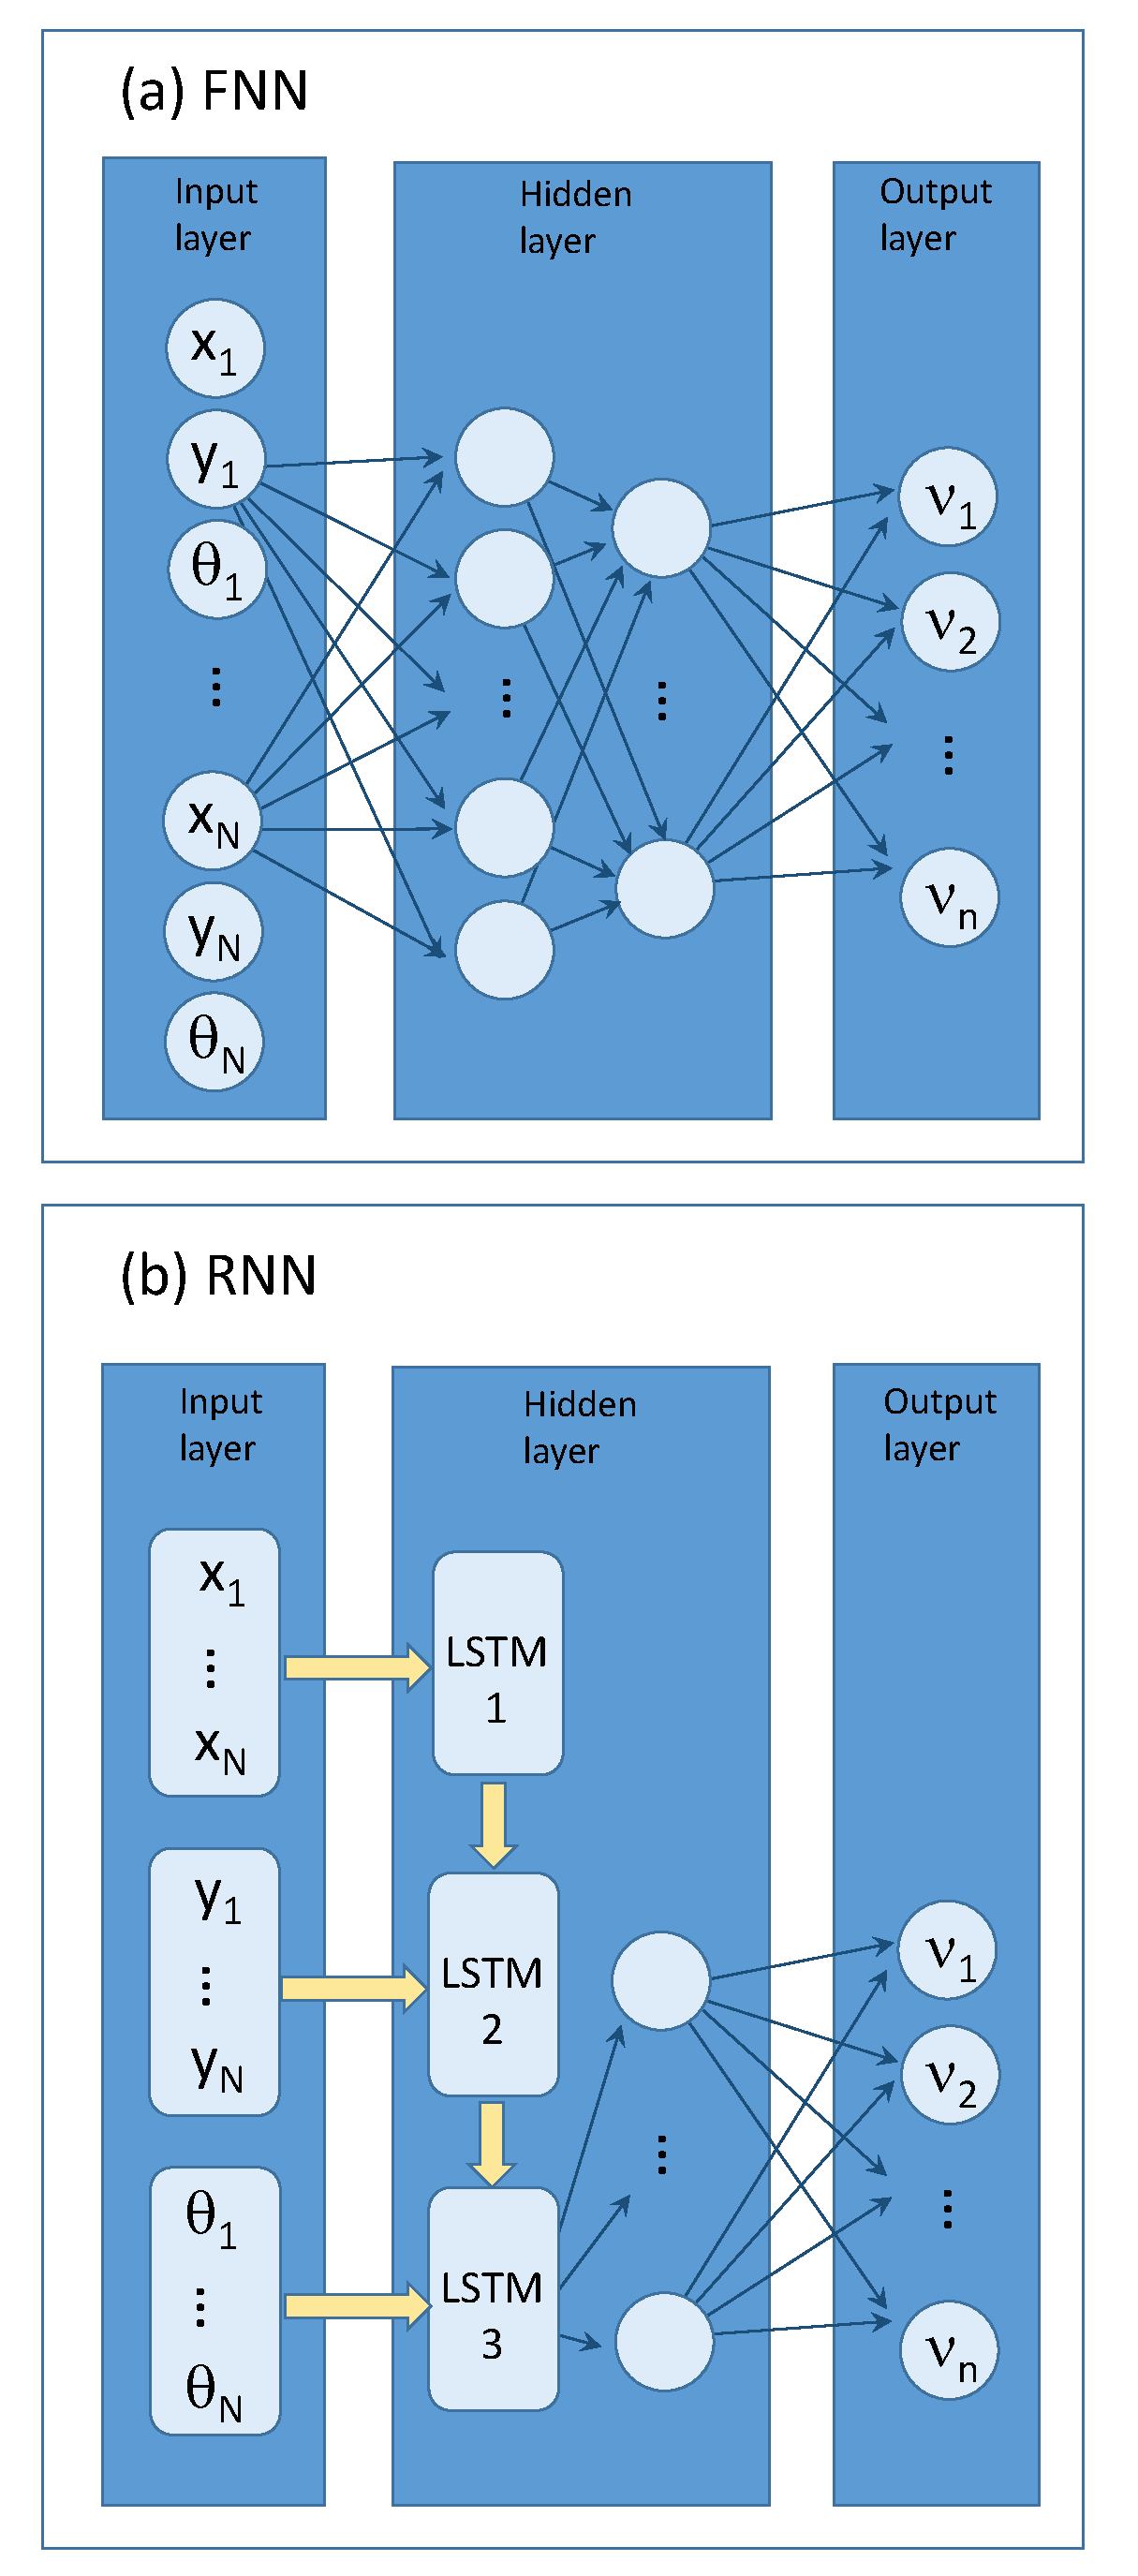
\includegraphics[width=0.5\textwidth]{./figs/FIG2.eps}
\caption{Schematics of (a) an FNN with two hidden layers and the sequence $(x_l, y_l, \theta_l)$ as input, where $l=1,2,...N$, and (b)
an RNN (unrolled) with the sequence $x_l$ ($l=1,2,...N$) as the input to the first LSTM block,
$y_l$ ($l=1,2,...N$) to the second LSTM block, and $\theta_l$ ($l=1,2,...N$) to the third LSTM block.
LSTM blocks also have LSTM-LSTM connections.
The final output of the two networks are $\nu_1, \nu_2, ..., \nu_n$, where $n$ is adjusted according to the type of features to be identified.}
\label{FIG2}
\end{figure}



\section{Application of FNN}\label{FNN}

First we review a few basic neural network concepts.
The main function of an NN is to read the system configuration through an input layer (e.g.\ an image, text, or sound bite), process the information in  hidden layers, and then generate an output. The output is often a classification estimation of the input, but may be another data structure (another image or sound bite for instance). In our case we look to classify system states through an FNN, sketched in Fig. \ref{FIG2}(a).
Each arrow (an ``edge'') represents a function call that connects nodes in different layers. These nodes, or ``perceptrons'', are inspired by the neuron model of the brain and are the building blocks of many neural networks, including the FNN, and though individually quite simple, complex functions can be represented by networking many perceptrons together \cite{rosenblatt}.
Going from input to output, data is repeatedly manipulated through function calls at each layer, with each containing their own network parameters --- usually referred to as weights and biases.
By varying network parameters the final output is consequently affected.
Training a network then involves optimizing the network's performance in producing the desirable output with respect to these network parameters.
%Multiple ``epochs'' are needed during the training, where w
Within one ``epoch'' the network is trained once on the selected dataset, and in general multiple epochs are needed for a network to converge to an acceptable performance.

A few technical details are provided.
We used a multilayer perceptron FNN of modest size, having two hidden layers: the first of size 128, and the second of size 32.
With the implementation of Tensorflow, exponential linear units were the chosen neurons for their proven effectiveness and quick learning \cite{elu,tensorflow}, and an early stopping technique determined sufficient training time \cite{nntricks}. Dropout was used at a 50\% drop rate to reduce overfitting the training \cite{dropout}.
The Adam algorithm was used for optimization \cite{adam}, and Softmax was applied to the output neurons to normalize the output set [see Appendix \ref{Supervise}].
For evaluating NN performance, a separate test dataset of images not seen during training is needed. A useful NN model needs to be able to correctly classify images it has not been trained on, otherwise it may merely have found a set of parameters that only work for the training set.

We used cross entropy $S$ as the cost function to measure the training quality on the training data set;
plotted as a function of epoch, we can see how the model learns over time and estimate its learning trajectory.
When the network is adequately trained, $S$ approaches 0. Another unique insight into the network's performance is the accuracy $A$, defined to measure the network performance on the unseen test set. An accuracy of 1 is scored for correct classification on the entire test set. Both $S$ and $A$ are quantitatively defined in Appendix \ref{Supervise}.

The physical system studied here is the defect states generated from the MC simulation of a two-dimensional off-lattice liquid-crystal model. In total, $N=784$ rod-like molecules of length $L$ are confined to a square box of dimensions $a\times a$. One can show that the parameter that drives the phase transition is the reduced density,
\begin{equation}\label{rho}
    \rho \equiv \frac{NL^2}{a^2}.
\end{equation}
Above the critical value $\rho^*$ the system is in a nematic state with directional ordering and below the critical value the system is in an isotropic state with random orientations (except those near the walls). The critical density $\rho^*\simeq 6.71$ can be estimated from a typical machine learning application, described in Appendix \ref{IN}.

\begin{figure}
\centering
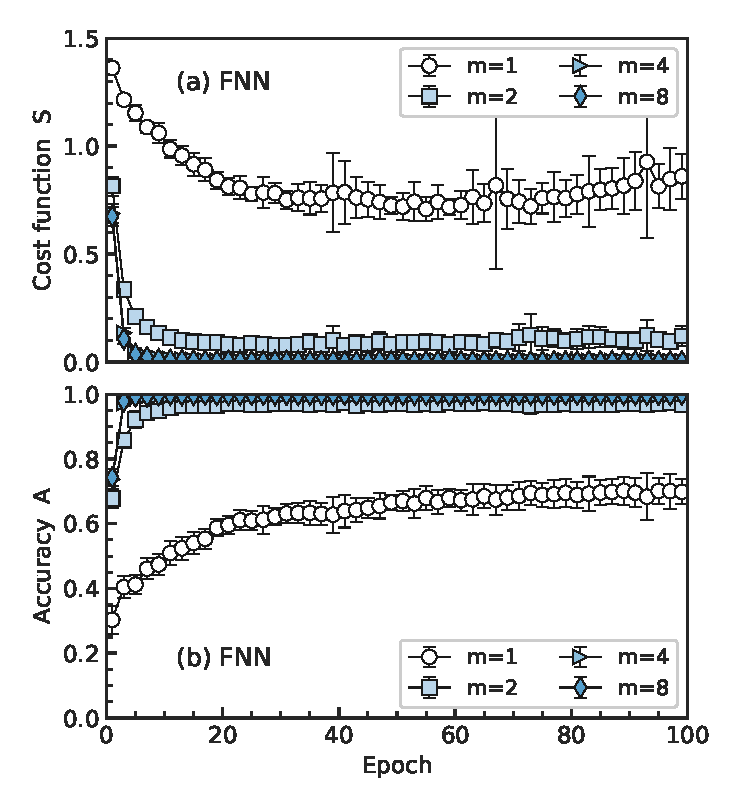
\includegraphics[width=0.8\textwidth]{./figs/FIG3AB.eps}
\caption{Cost function $S$ and accuracy $A$, defined on the training and test datasets respectively, monitored on an FNN as functions of epoch step. Symbols in the plots represent the averaged $S$ and $A$ produced from 20 repeated training runs, from which errorbars are also estimated. Circles, squares, triangles, and diamonds correspond to the degrees of coarse-graining in the presorting procedure used: $m=1$ (unsorted raw data), $2$, 4, and 8, respectively. For coarse-graining, the original simulation box in Fig.\ \ref{FIG1}(e)-(h) is divided into $m\times m$ cells [see Section \ref{FNN}].
}
\label{fnn_SA}
\end{figure}

\begin{figure}
\centering
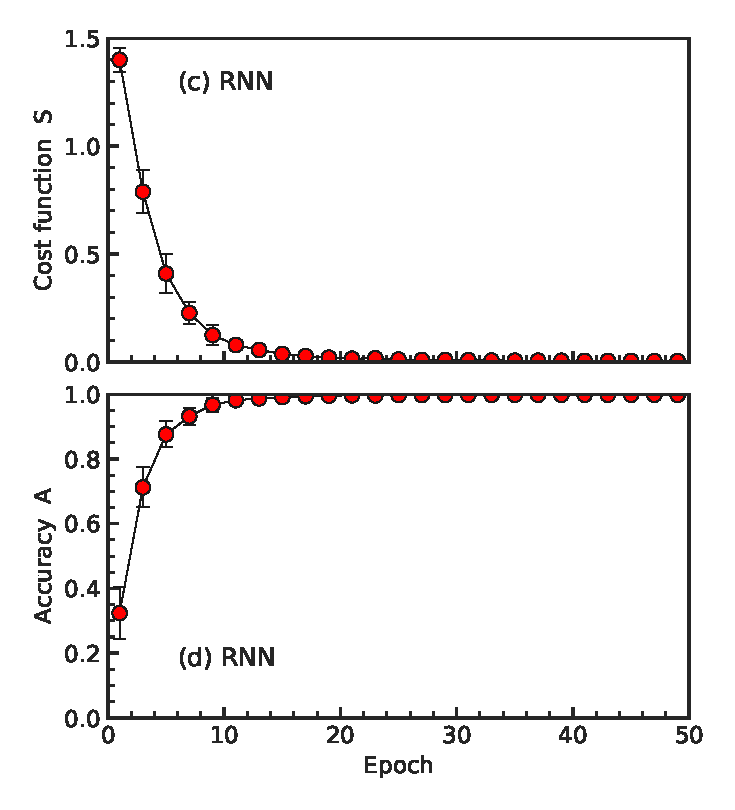
\includegraphics[width=0.8\textwidth]{./figs/FIG3CD.eps}
\caption{Cost function $S$ and accuracy $A$, defined on the training and test datasets respectively, monitored an RNN as functions of epoch step. Symbols in the plots represent the averaged $S$ and $A$ produced from 20 repeated training runs, from which errorbars are also estimated.
}
\label{rnn_SA}
\end{figure}

Our main concern here is identifying the defect states, not the isotropic-to-nematic phase transition itself.
Within the nematic state, the system can display a stable D-defect pattern, or can be trapped in the free energy minima corresponding to one of the X-, T-, or U-defect patterns, due to the finite confinement effects. The nature of the metastability has been recently addressed extensively in Refs.\ \cite{Galanis2006,Mulder2011,Lewis2014,Cortes2017,Tsakonas2007,Luo2012,chen2013rods,Mulder2015}.
In order to explore the best machining learning techniques in identifying the defect states, we established a database from the MC simulations at a fixed  $\rho=19.63$ (produced by setting $a=6.32L$). The relatively high $\rho$  enables the trapping of the metastable defect patterns during simulation runs. In total, $4400$ independent configurational snapshots were collected for each of the defect states [see Appendix \ref{MC}].
%
%To build up datasets a relatively high density of $\rho=19.63$ was used so the different defect patterns could maintain their form as they are metastable at lower densities. For each pattern $4400$ independent snapshots were collected [see Appendix \ref{MC}].
For each configuration, $4000$ were used for training and the remainder for testing. The raw dataset of each snapshot contained data ordered by the label of molecules, $l$, and followed by $[x_l,y_l,\theta_l]$.

%The MC parameters for the DTUX sets were chosen so as to be in a favorable region for both $U$ and $T$ states, as predicted by Yao \cite{yao}. We chose a box size of edge length $a=6.32$, rod length of unity, and number of rods $N=28^2$, yielding a reduced density $\rho^*=19.63$. This region, though favorable, was still only metastable and relaxing for much longer than $10^5$ Monte Carlo sweeps (where one sweep attempts to move each rod) would inevitably tend towards the more preferred D state. In accounting for this, after $10^5$ sweeps, the state snapshot would be recorded, the system would be reinitialized, and the process would repeat. This additionally ensured no temporal correlation among snapshots.

A naive approach would be directly taking an FNN for identifying these defect states, feeding the raw $[x,y,\theta]$ data into the $3N$ input nodes, and training the network to recognize the four different topologies by supervised learning [see Appendix \ref{Supervise}].
This approach has seen success in learning phase transitions of Ising systems \cite{carras}, polymer systems \cite{wei}, and the XY model \cite{beach}. However, this method showed a pronounced failure in the current application.
As we show in Fig.~\ref{xtud-all}(a), indicated as $m=1$, this approach does not come close to an acceptable performance, producing a plateau in an undiminishing cost. In addition, $A$ reaches a plateau at an unsatisfactory level of approximately $60\%$.

Why is this so?
One of the essential features the network needs to learn for these defect configurations is the correlation between the position of a topological defect and the molecular orientation in the vicinity of the defect. A typical raw snapshot datafile records the $[x,y,\theta]$ data sequentially according to the order of the label of the rodlike molecules $l$. Because there is no a priori knowledge of which molecules show up in the defect regions, the labels of the defect-region molecules differ from file to file. Indeed, in a statistically independent set of files, such as the ones produced here from different initial conditions [see Appendix \ref{MC}], there are no label-position correlations of the defect-region molecules among the learning data files.
This all addresses a crucial, but often unnoticed, aspect of image classification: by filling input vectors in a positionally sorted fashion [Fig.~ \ref{FIG1}(a),(b)], positional information, and indeed its correlation to whichever feature is being written to the input vector, is consequently encoded. If this sorting is destroyed, even if we give the positions (such as $[x,y]$
) as part of the input data, the position-feature (e.g.\ $\theta$) correlation is destroyed. This unseen property, and its essential importance can also be demonstrated via the digit recognition problem in Appendix \ref{AppMNIST}.

Hence, the key information is the position sorting in the initial data input, as the FNN relates features with the ordering of the input data. We develop the following coarse-graining procedure to train an FNN in identifying liquid crystal defects shown in Fig.~\ref{FIG1}.

The confinement box (Fig.~\ref{FIG1}) is divided into $m\times m$ cells, where $m$ is an integer. The cells are labeled $M=1,2,...m\times m$ horizontally, row by row.
The raw data in every snapshot is presorted according to their $[x,y]$ coordinates so that molecules belonging to the $M=1$ cell show up first, $M=2$ cell show up second, etc. Within a cell, the order of data is still random and no further presorting is made. The $m=1$ case returns to the raw data format. By the end, the order of appearance of molecular information is no longer according to $l$, but, according to $M$ for all coarse-graining degree $m\ge 2$. The presorted data is then used in supervised training.

The presorting procedure works well with an FNN. Figures \ref{fnn_SA}(a) and (b) show how the cost function and accuracy quickly approach the ideal value of $0$ and $1$ respectively, as we presort the data beyond $m=2$.
In the case of $m=4, 8$, less than 20 epochs (surprisingly short) are needed to adequately train the FNN. This can be attributed to the defect patterns in Fig.\ \ref{FIG1} themselves. By dividing the square box in $m=4$ cells, for example, one can already distinguish the defect structures, by ignoring fine details inside a single cell.
Of course,  in general we expect that the degree of coarse-graining, $m$, needs to increase for a more complicated defect pattern with more defect features.

In summary, to effectively train an FNN to identify features in an image or simulation data file, the ordering of data points (pixels in image, spins in the Ising model, and rodlike molecules in the current study) contains vital information of the data. An off-lattice model usually produces data with a random order and it must be presorted according their approximate $[x,y]$ coordinates, if we are looking for the correlation between coordinates and the physical features.

\section{Application of RNN}\label{RNN}

A typical structure of the recurrent neutral network (RNN) is represented in Fig.~\ref{FIG2}(b). The crux of this RNN is the long short-term memory (LSTM) cell module \cite{lstm}. An RNN can be made with different types of modules, but LSTM is a popular choice and is well-sufficient for this work. Except for the first block, an LSTM cell has two input channels: an LSTM-external connection
to new raw data from the system to be studied,
and an LSTM-LSTM connection, taking its own output and internal weights from the previous step as input, hence the recurrent aspect. Schematically, it helps to show a series of LSTM cells for each raw data input. %, but there is really only one.
To complete the RNN, a single layer of perceptrons is appended to act as
a final interpretive layer of the LSTM output, which compresses the large LSTM output to the smaller prediction output $(\nu_1, \nu_2, ..., \nu_n)$.

A typical application of an RNN is comparing a time series of data.
An LSTM cell can take a complete data file and at each iteration of input, consider the new raw data together with its own previous state simultaneously. That is, an LSTM establishes data correlations with those fed into earlier cell states through LSTM-LSTM connections.
%A popular application of RNNs is speech recognition, where a long series of connected LSTM blocks are used; if one uses $i$ to denote LSTM blocks sequentially, then the input to the $i$th LSTM block is a complete dataset occurred at time frame $t_i$; the time series $...t_{i-2}, t_{i-1}, t_i$ of a speech record can then be processed with time-correlation.
In its composition, like an FNN, an RNN (including the LSTM) is still merely an ensemble of floating-point network parameters.
The logic of supervised training is the same here in comparison with an FNN: determination of the network parameters through optimization of a cost function. The RNN can be coded in terms of Tensorflow libraries efficiently.


Here we demonstrate a novel usage of an RNN in condensed matter systems. Exploiting its ability to correlate physical features through LSTM blocks, we adopt a triple iterative structure shown in Fig.\ \ref{FIG2}(b) to find the correlation between the spatial coordinates $x$, $y$ and the orientational coordinate $\theta$. The raw data
has a line-by-line format $[l, x_l, y_l, \theta_l]$, where $l=1,..., N$. The three main features, $x_l, y_l$ and $\theta_l$ are input into the network model iteratively through the LSTM-external layer, one after another. As a technical note, we used a rather small RNN having only a single layer LSTM of 64 hidden neurons, and a single perceptron layer of 128 neurons. Dropout, Adam optimization, and early stopping were again used throughout the supervised training \cite{dropout,nntricks,adam}.

The performance of this RNN is exceptionally good in identifying the defect states. Figures \ref{rnn_SA}(c) and (d) demonstrate that within an initial 20 epochs, our RNN efficiently captures the main features of the four defect states, evaluated on an unseen test dataset. We stress here that unlike the procedure used to produce Figs. \ref{fnn_SA}(a) and (b), we used the raw, unsorted data as the input on our RNN experiment.

%It is not surprising because RNN is known to capture temporal correlations, and it is adopted here to capture spatial correlations.


%The correlation is achieved thanks to the sequential feeding of the $x,y$, and $\theta$ features. Like the FNN, the LSTM has an internal set of weights that are trained while optimizing the model. While reading the sequence of inputs, the LSTM also maintains a ``cell state''. This cell state is updated with each input, first on the $x$ data, again on the $y$ data, and a third time on the $\theta$ data. Additionally, updating the cell state not only depends on what current information is being fed, but also on the previous cell state (hence the recurrent attribute). For example, we may consider two images that have the same value $\theta_i$ in the $i$th position (or even an identical $\theta$ vector) but different $[x_i,y_i]$ coordinates. The structure of the RNN naturally correlates $\theta_i$ to the position coordinates also in their $i$th positions and so interprets the angular information properly.

%===========================








%---------------------------
% END MATERIAL
%---------------------------

% B I B L I O G R A P H Y
% --------------------------

% The following statement selects the style to use for references.  It controls the sort order of the entries in the bibliography and also the formatting for the in-text labels.
\bibliographystyle{plain}
% This specifies the location of the file containing the bibliographic information.  
% It assumes you're using BibTeX (if not, why not?).
\cleardoublepage % This is needed if the book class is used, to place the anchor in the correct page, because the bibliography will start on its own page. Use \clearpage instead if the document class uses the "oneside" argument

\phantomsection  % With hyperref package, enables hyperlinking from the table of contents to bibliography             
% The following statement causes the title "References" to be used for the bibliography section:
\renewcommand*{\bibname}{References}

% Add the References to the Table of Contents
\addcontentsline{toc}{chapter}{\textbf{References}}

\bibliography{thesis}
% The following statement causes the specified references to be added to the bibliography% even if they were not cited in the text. The asterisk is a wildcard that causes all entries in the bibliographic database to be included (optional).
\nocite{*}

% The \appendix statement indicates the beginning of the appendices.
\appendix
% Add a title page before the appendices and a line in the Table of Contents
\chapter*{APPENDICES}
\addcontentsline{toc}{chapter}{APPENDICES}
\input{appendix}
%======================================================================

\end{document}
